% Options for packages loaded elsewhere
\PassOptionsToPackage{unicode}{hyperref}
\PassOptionsToPackage{hyphens}{url}
%
\documentclass[
]{article}
\usepackage{amsmath,amssymb}
\usepackage{lmodern}
\usepackage{iftex}
\ifPDFTeX
  \usepackage[T1]{fontenc}
  \usepackage[utf8]{inputenc}
  \usepackage{textcomp} % provide euro and other symbols
\else % if luatex or xetex
  \usepackage{unicode-math}
  \defaultfontfeatures{Scale=MatchLowercase}
  \defaultfontfeatures[\rmfamily]{Ligatures=TeX,Scale=1}
\fi
% Use upquote if available, for straight quotes in verbatim environments
\IfFileExists{upquote.sty}{\usepackage{upquote}}{}
\IfFileExists{microtype.sty}{% use microtype if available
  \usepackage[]{microtype}
  \UseMicrotypeSet[protrusion]{basicmath} % disable protrusion for tt fonts
}{}
\makeatletter
\@ifundefined{KOMAClassName}{% if non-KOMA class
  \IfFileExists{parskip.sty}{%
    \usepackage{parskip}
  }{% else
    \setlength{\parindent}{0pt}
    \setlength{\parskip}{6pt plus 2pt minus 1pt}}
}{% if KOMA class
  \KOMAoptions{parskip=half}}
\makeatother
\usepackage{xcolor}
\usepackage[margin=1in]{geometry}
\usepackage{color}
\usepackage{fancyvrb}
\newcommand{\VerbBar}{|}
\newcommand{\VERB}{\Verb[commandchars=\\\{\}]}
\DefineVerbatimEnvironment{Highlighting}{Verbatim}{commandchars=\\\{\}}
% Add ',fontsize=\small' for more characters per line
\usepackage{framed}
\definecolor{shadecolor}{RGB}{248,248,248}
\newenvironment{Shaded}{\begin{snugshade}}{\end{snugshade}}
\newcommand{\AlertTok}[1]{\textcolor[rgb]{0.94,0.16,0.16}{#1}}
\newcommand{\AnnotationTok}[1]{\textcolor[rgb]{0.56,0.35,0.01}{\textbf{\textit{#1}}}}
\newcommand{\AttributeTok}[1]{\textcolor[rgb]{0.77,0.63,0.00}{#1}}
\newcommand{\BaseNTok}[1]{\textcolor[rgb]{0.00,0.00,0.81}{#1}}
\newcommand{\BuiltInTok}[1]{#1}
\newcommand{\CharTok}[1]{\textcolor[rgb]{0.31,0.60,0.02}{#1}}
\newcommand{\CommentTok}[1]{\textcolor[rgb]{0.56,0.35,0.01}{\textit{#1}}}
\newcommand{\CommentVarTok}[1]{\textcolor[rgb]{0.56,0.35,0.01}{\textbf{\textit{#1}}}}
\newcommand{\ConstantTok}[1]{\textcolor[rgb]{0.00,0.00,0.00}{#1}}
\newcommand{\ControlFlowTok}[1]{\textcolor[rgb]{0.13,0.29,0.53}{\textbf{#1}}}
\newcommand{\DataTypeTok}[1]{\textcolor[rgb]{0.13,0.29,0.53}{#1}}
\newcommand{\DecValTok}[1]{\textcolor[rgb]{0.00,0.00,0.81}{#1}}
\newcommand{\DocumentationTok}[1]{\textcolor[rgb]{0.56,0.35,0.01}{\textbf{\textit{#1}}}}
\newcommand{\ErrorTok}[1]{\textcolor[rgb]{0.64,0.00,0.00}{\textbf{#1}}}
\newcommand{\ExtensionTok}[1]{#1}
\newcommand{\FloatTok}[1]{\textcolor[rgb]{0.00,0.00,0.81}{#1}}
\newcommand{\FunctionTok}[1]{\textcolor[rgb]{0.00,0.00,0.00}{#1}}
\newcommand{\ImportTok}[1]{#1}
\newcommand{\InformationTok}[1]{\textcolor[rgb]{0.56,0.35,0.01}{\textbf{\textit{#1}}}}
\newcommand{\KeywordTok}[1]{\textcolor[rgb]{0.13,0.29,0.53}{\textbf{#1}}}
\newcommand{\NormalTok}[1]{#1}
\newcommand{\OperatorTok}[1]{\textcolor[rgb]{0.81,0.36,0.00}{\textbf{#1}}}
\newcommand{\OtherTok}[1]{\textcolor[rgb]{0.56,0.35,0.01}{#1}}
\newcommand{\PreprocessorTok}[1]{\textcolor[rgb]{0.56,0.35,0.01}{\textit{#1}}}
\newcommand{\RegionMarkerTok}[1]{#1}
\newcommand{\SpecialCharTok}[1]{\textcolor[rgb]{0.00,0.00,0.00}{#1}}
\newcommand{\SpecialStringTok}[1]{\textcolor[rgb]{0.31,0.60,0.02}{#1}}
\newcommand{\StringTok}[1]{\textcolor[rgb]{0.31,0.60,0.02}{#1}}
\newcommand{\VariableTok}[1]{\textcolor[rgb]{0.00,0.00,0.00}{#1}}
\newcommand{\VerbatimStringTok}[1]{\textcolor[rgb]{0.31,0.60,0.02}{#1}}
\newcommand{\WarningTok}[1]{\textcolor[rgb]{0.56,0.35,0.01}{\textbf{\textit{#1}}}}
\usepackage{longtable,booktabs,array}
\usepackage{calc} % for calculating minipage widths
% Correct order of tables after \paragraph or \subparagraph
\usepackage{etoolbox}
\makeatletter
\patchcmd\longtable{\par}{\if@noskipsec\mbox{}\fi\par}{}{}
\makeatother
% Allow footnotes in longtable head/foot
\IfFileExists{footnotehyper.sty}{\usepackage{footnotehyper}}{\usepackage{footnote}}
\makesavenoteenv{longtable}
\usepackage{graphicx}
\makeatletter
\def\maxwidth{\ifdim\Gin@nat@width>\linewidth\linewidth\else\Gin@nat@width\fi}
\def\maxheight{\ifdim\Gin@nat@height>\textheight\textheight\else\Gin@nat@height\fi}
\makeatother
% Scale images if necessary, so that they will not overflow the page
% margins by default, and it is still possible to overwrite the defaults
% using explicit options in \includegraphics[width, height, ...]{}
\setkeys{Gin}{width=\maxwidth,height=\maxheight,keepaspectratio}
% Set default figure placement to htbp
\makeatletter
\def\fps@figure{htbp}
\makeatother
\setlength{\emergencystretch}{3em} % prevent overfull lines
\providecommand{\tightlist}{%
  \setlength{\itemsep}{0pt}\setlength{\parskip}{0pt}}
\setcounter{secnumdepth}{5}
\pagenumbering{gobble}
\usepackage{subfig}
\usepackage[labelsep=period]{caption}
\usepackage[labelfont=bf]{caption}
\renewcommand{\and}{\\}
\ifLuaTeX
  \usepackage{selnolig}  % disable illegal ligatures
\fi
\IfFileExists{bookmark.sty}{\usepackage{bookmark}}{\usepackage{hyperref}}
\IfFileExists{xurl.sty}{\usepackage{xurl}}{} % add URL line breaks if available
\urlstyle{same} % disable monospaced font for URLs
\hypersetup{
  pdftitle={Número de pasajeros en el Puerto de Barcelona (2012-2019)},
  pdfauthor={Garcia Sató, Pol; Nualart Sanz, Arnau},
  hidelinks,
  pdfcreator={LaTeX via pandoc}}

\title{Número de pasajeros en el Puerto de Barcelona (2012-2019)}
\usepackage{etoolbox}
\makeatletter
\providecommand{\subtitle}[1]{% add subtitle to \maketitle
  \apptocmd{\@title}{\par {\large #1 \par}}{}{}
}
\makeatother
\subtitle{Segona pràctica Anàlisi de Series Temporals}
\author{Garcia Sató, Pol \and Nualart Sanz, Arnau}
\date{02 enero, 2023}

\begin{document}
\maketitle

\renewcommand{\contentsname}{Índex}
\renewcommand{\figurename}{Figura}
\renewcommand{\tablename}{Taula}

\captionsetup{width=.75\textwidth}

\begin{longtable}[]{@{}
  >{\raggedright\arraybackslash}p{(\columnwidth - 2\tabcolsep) * \real{0.5000}}
  >{\raggedright\arraybackslash}p{(\columnwidth - 2\tabcolsep) * \real{0.5000}}@{}}
\toprule()
\endhead

\includegraphics[width=0.4\textwidth,height=\textheight]{C:/Users/polgs/Desktop/Grau estadística UB/4rt de carrera/1er Quadrimestre/AnalisisSeriesTemporals/Entrega2/Imatges/ub.png}
&

\includegraphics[width=0.4\textwidth,height=\textheight]{C:/Users/polgs/Desktop/Grau estadística UB/4rt de carrera/1er Quadrimestre/AnalisisSeriesTemporals/Entrega2/Imatges/upc.png} \\
\bottomrule()
\end{longtable}


\includegraphics[width=0.4\textwidth,height=\textheight]{C:/Users/polgs/Desktop/Grau estadística UB/4rt de carrera/1er Quadrimestre/AnalisisSeriesTemporals/Entrega2/Imatges/ub.png}


\includegraphics[width=0.4\textwidth,height=\textheight]{C:/Users/polgs/Desktop/Grau estadística UB/4rt de carrera/1er Quadrimestre/AnalisisSeriesTemporals/Entrega2/Imatges/upc.png}

\vspace{60mm}

\renewcommand{\contentsname}{Índex}
\renewcommand{\figurename}{Figura}
\renewcommand{\tablename}{Taula}

\begin{longtable}[]{@{}l@{}}
\toprule()
\endhead
```\{=tex\} \\
\textbackslash begin\{center\} \\
El objetivo de este informe es ver el comportamiento del número de
pasajeros en el puerto de Barcelona durante los años 2012 - 2019 y hacer
una predicción para el período 2020 - 2022 si no se tuvieran en cuenta
los efectos causados por la pandemia del SARS-CoV-2. \\
Se observa que los datos presentan tendencia creciente y estacionalidad
multiplicativa. Es decir, con el paso de los años la demanda fue
aumentando. Además, hay un claro patrón estacional que muestra que en
los meses de verano el número es superior a los meses de otoño e
invierno. \\
En cuanto a la predicción, la demanda sigue aumentando de manera
multiplicativa y siguiendo el mismo patrón estacional. \\
\textbackslash end\{center\} \\
``` \\
\bottomrule()
\end{longtable}

\newpage

\pagebreak

\tableofcontents

\pagebreak

\hypertarget{introducciuxf3}{%
\section{Introducció}\label{introducciuxf3}}

\hypertarget{descripciuxf3n-del-entorno-y-el-problema---motivaciuxf3n-del-trabajo}{%
\subsection{Descripción del entorno y el problema - motivación del
trabajo}\label{descripciuxf3n-del-entorno-y-el-problema---motivaciuxf3n-del-trabajo}}

Desde el estallido de la pandemia del SARS-CoV-2 las preferencias de la
población respecto a sus destinos vacacionales parecen haber cambiado.
Actualmente, los viajeros están más interesados en lugares naturales, al
aire libre, debido a que en la época del confinamiento mucha parte de la
población se sintió agobiada dentro de sus hogares. Adicionalmente, los
españoles se han centrado en un turismo nacional debido a la situación
de crisis sanitaria que estamos viviendo. Así pues, el número de
pasajeros en el Puerto de Barcelona puede haber disminuido drásticamente
ya que los cruceros son espacios cerrados y suelen ser vacaciones
internacionales.

El objetivo principal de este informe es ver cuál era el comportamiento
del número de pasajeros en el Puerto de Barcelona, ya sean de cruceros
como de ferris, en los años anteriores a la pandemia. De esta manera se
podrá ver de manera correcta la tendencia creciente que se tenía antes
de la crisis sin tener en cuenta la posible caída debida a la pandemia.

Para la elección de los años analizados, se ha evitado estudiar aquellos
momentos temporales en los que había un factor condicionante. Por tanto,
los datos tomados dejan fuera la crisis económica del 2008 y la pandemia
del 2020. También tendremos en cuenta que a principios del 2012 hubo el
desastre de la naviera italiana Costa Concordia con 32 muertos, lo cual
hizo que hubiera un descenso significativo en el número de pasajeros en
los cruceros del Mediterráneo. Teniendo esto en cuenta, solo se han
seleccionado los datos mensuales pertenecientes al espacio temporal
comprendido entre 2012 y 2019, ambos períodos incluidos.

\smallskip

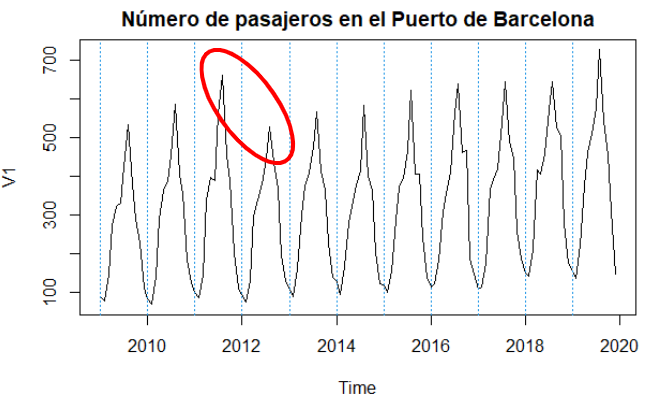
\includegraphics[width=0.5\textwidth,height=\textheight]{C:/Users/polgs/Desktop/Grau estadística UB/4rt de carrera/1er Quadrimestre/AnalisisSeriesTemporals/Entrega2/Imatges/grafic.png}

\hypertarget{definiciuxf3n-precisa-de-la-variable}{%
\subsection{Definición precisa de la
variable}\label{definiciuxf3n-precisa-de-la-variable}}

La variable a estudiar es el número de pasajeros que llegan al Puerto de
Barcelona durante el periodo ya comentado anteriormente. Cabe destacar
que esta variable recoge tanto el número de llegadas internas
(nacionales) como externas (internacionales).

\hypertarget{descripciuxf3n-de-la-fuente-de-informaciuxf3n}{%
\subsection{Descripción de la fuente de
información}\label{descripciuxf3n-de-la-fuente-de-informaciuxf3n}}

Los datos han sido extraídos de los casos propuestos del repositorio que
precisamos en el CV de la UB. Provienen de la web del Ministerio del
Fomento (\url{http://www.fomento.gob.es}) en el apartado Ministerio de
Fomento / Marítimo / Información Estadística y corresponden al número de
pasajeros que llegan al Puerto de Barcelona.

\hypertarget{resumen-de-la-estructura-del-trabajo}{%
\subsection{Resumen de la estructura del
trabajo}\label{resumen-de-la-estructura-del-trabajo}}

El estudio sigue el siguiente esquema:

\begin{itemize}
\tightlist
\item
  \emph{Aplicación empírica}
\end{itemize}

En este apartado se observan cuáles son las características principales
de la serie (media, varianza, tendencia, estacionalidad, residuos,. . .
). Es decir, se analiza descriptivamente la serie para así tener un
conocimiento previo de los datos.

\begin{itemize}
\tightlist
\item
  \emph{Metodología de alisado}
\end{itemize}

A partir del análisis realizado en el apartado anterior se decide qué
tipo de serie se ajusta mejor a nuestros datos. A partir de aquí, se
hace una predicción para observar cuál sería el número de viajeros en
alojamientos rurales en los próximos años si no existiera ningún factor
condicionante que actuará como brecha, en el caso expuesto, si no
existiera la pandemia del Covid-19.

\medskip

\hypertarget{aplicaciuxf3n-empuxedrica}{%
\section{Aplicación empírica}\label{aplicaciuxf3n-empuxedrica}}

\hypertarget{anuxe1lisis-descriptivo-de-la-serie}{%
\subsection{Análisis descriptivo de la
serie}\label{anuxe1lisis-descriptivo-de-la-serie}}

El análisis descriptivo de los datos seleccionados comenzará con una
herramienta visual, un gráfico que permitirá observar la distribución de
éstos a lo largo de los 8 años estudiados. El gráfico temporal tiene la
siguiente forma:

\begin{center}\includegraphics{PracticaAST_files/figure-latex/unnamed-chunk-1-1} \end{center}

Como ya se explicó con detalle en la práctica 1, la serie estudiada
presenta una tendencia creciente y una estacionalidad multiplicativa de
orden s = 12.

\hypertarget{identificaciuxf3n-del-modelo}{%
\subsection{Identificación del
modelo}\label{identificaciuxf3n-del-modelo}}

\hypertarget{transformaciuxf3n-de-la-serie-temporal-en-una-serie-estacionaria}{%
\subsubsection{Transformación de la serie temporal en una serie
estacionaria}\label{transformaciuxf3n-de-la-serie-temporal-en-una-serie-estacionaria}}

Para que la serie estudiada sea estacionaria estudiaremos que la
varianza sea constante, que no exista componente estacional y que
presente una media constante.

\textbf{Varianza constante}

Se dispone de dos soportes gráficos que permiten ver si la varianza de
la serie es constante o no: \emph{Gráfico medias vs varianzas} y
\emph{Boxplot por periodos}.

\begin{center}\includegraphics{PracticaAST_files/figure-latex/unnamed-chunk-2-1} \end{center}

En el primer gráfico podemos observar que, a medida que aumenta la
media, también lo hace la varianza. Lo mismo podemos decir en el segundo
gráfico boxplot, donde el rango intercuartílico aumenta al mismo paso
que aumenta el nivel de la serie.

Entonces podemos concluir que la varianza de la serie no es constante.
Para que lo sea, usaremos una transformación logarítmica graficando de
nuevo los datos.

\begin{center}\includegraphics{PracticaAST_files/figure-latex/unnamed-chunk-3-1} \end{center}

Ahora sí podríamos decir que la varianza de la serie se ha estabilizado
al aplicar la transformación logaritmica.

\medskip

\textbf{Patrón estacional}

Para saber si existe patrón estacional usaremos la función
\texttt{monthplot}, que calcula la media en cada orden estacional. En
nuestro caso, mensualmente.

\begin{center}\includegraphics{PracticaAST_files/figure-latex/unnamed-chunk-4-1} \end{center}

Vemos claramente que hay irregularidades en la media para cada mes, ya
que no hay equilibrio en sus líneas horizonales. Por lo que podemos
decir que la serie presenta un patrón estacional de orden s=12, como se
ha dicho anteriormente. Para poder eliminarlo, se realiza una
diferenciación estacional (D = 1), es decir, se restan las observaciones
del patrón estacional anterior. Por tanto, se eliminarán S = 12
observaciones, las 12 primeras.

Volvemos a utilizar la función \texttt{monthplot} sobre la serie
diferenciada estacionalmente para comprobar que se haya eliminado el
patrón estacional.

\begin{center}\includegraphics{PracticaAST_files/figure-latex/unnamed-chunk-6-1} \end{center}

Vemos que, efectivamente, se han estabilizado las medias de cada mes,
por lo que podemos afirmar que hemos eliminado el patrón estacional.

\medskip

\textbf{Media constante}

Se obtiene el gráfico temporal de la serie en escala logarítmica y con
una diferenciación estacional.

\begin{center}\includegraphics{PracticaAST_files/figure-latex/unnamed-chunk-7-1} \end{center}

Podemos ver que la media de la serie parece constante pero no llega al
valor nulo deseado. Por ello, haremos una diferenciación regular (d=1) y
volveremos a graficar la serie para verificar que es 0.

\begin{center}\includegraphics{PracticaAST_files/figure-latex/unnamed-chunk-9-1} \end{center}

Ahora podemos ver como la media sí tiene valor nulo pero para comprobar
que la serie no presenta sobrediferenciación compararemos las varianzas
de las tres transformaciones.

\begin{verbatim}
##          V1
## V1 0.378022
\end{verbatim}

\begin{verbatim}
##            V1
## V1 0.01363138
\end{verbatim}

\begin{verbatim}
##            V1
## V1 0.01699842
\end{verbatim}

\begin{longtable}[]{@{}llll@{}}
\toprule()
Modelo & lnserie & d12lnserie & d1d12lnserie \\
\midrule()
\endhead
Varianza & 0.378022 & 0.0136314 & 0.0169984 \\
\bottomrule()
\end{longtable}

Se observa que la segunda serie presenta una menor varianza pero no se
aleja significativamente de la tercera y, como deseábamos tener un valor
nulo de la media, nos quedamos con esta.

\hypertarget{identificaciuxf3n-de-modelos-pausibles}{%
\subsubsection{Identificación de modelos
pausibles}\label{identificaciuxf3n-de-modelos-pausibles}}

Para identificar algunos modelos graficamos el ACF y el PACF de la serie
estacionaria. En el siguiente gráfico se muestra en color rojo los ``s''
rezagos estacionales de la función (P)ACF. En negro, todos los rezagos
regulares.

\begin{center}\includegraphics{PracticaAST_files/figure-latex/unnamed-chunk-11-1} \end{center}

Podemos confirmar que se ha llegado a la serie estacionaria ya que los
valores de ACF disminuyen hacia el 0.

Observando las gráficas se concluye que:

\begin{itemize}
\item
  \emph{Opciones para la parte regular}: MA(1), AR(2)
\item
  \emph{Opciones para la parte estacional}: SMA(1), SAR(1) con S=12
\end{itemize}

Todas ellas con las diferenciaciones aplicadas, una regular (d = 1) y
otra estacional (D = 1 con S = 12).

Así pues, se obtienen 4 posibles combinaciones, 4 modelos propuestos.

\pagebreak

\hypertarget{forma-compacta-y-usando-el-operador-de-retardo-b-de-los-modelos-identificados}{%
\subsubsection{Forma compacta y usando el operador de retardo B de los
modelos
identificados}\label{forma-compacta-y-usando-el-operador-de-retardo-b-de-los-modelos-identificados}}

\(W_t = (1-B)^d(1-B^S)^D ln(W_t)\)

\medskip

\underline{Modelo 1:} \(MA(1)SMA(1)_{12}\) para \(W_t\)

Forma compacta de modelo ARIMA para \(ln(X_t)\)

\((1-B)(1-B^{12}) ln(X_t) = \theta_1(B)\Theta_1(B^{12})Z_t, d = 1,\; y \; D = 1 \; con \; S = 12\)

Sustituyendo cada polinomio característico se obtiene:

\((1-B)(1-B^{12}) ln(X_t) = (1+\theta_1B)(1+\Theta_1B^{12})Z_t\)

\medskip

\underline{Modelo 2:} \(AR(2)SMA(1)_{12}\) para \(W_t\)

Forma compacta de modelo ARIMA para \(ln(X_t)\)

\(\phi_2(B) (1-B)(1-B^{12}) ln(X_t) = \Theta_1(B^{12})Z_t, d = 1,\; y \; D = 1 \; con \; S = 12\)

Sustituyendo cada polinomio característico se obtiene:

\((1-\phi_1B-\phi_2B^2)(1-B)(1-B^{12}) ln(X_t) = (1+\Theta_1B^{12})Z_t\)

\medskip

\underline{Modelo 3:} \(MA(1)SAR(1)_{12}\) para \(W_t\)

Forma compacta de modelo ARIMA para \(ln(X_t)\)

\((1-\Phi_1B^{12})(1-B)(1-B^{12}) ln(X_t) =\theta_1(B)Z_t, d = 1,\; y \; D = 1 \; con \; S = 12\)

Sustituyendo cada polinomio característico se obtiene:

\((1-\Phi_1B^{12})(1-B)(1-B^{12}) ln(X_t) = (1+\theta_1B)Z_t\)

\medskip

\underline{Modelo 4:} \(AR(2)SAR(1)_{12}\) para \(W_t\)

Forma compacta de modelo ARIMA para \(ln(X_t)\)

\(\phi_2(B)(1-\Phi_1B^{12})(1-B)(1-B^{12}) ln(X_t) = Z_t, d = 1,\; y \; D = 1 \; con \; S = 12\)

Sustituyendo cada polinomio característico se obtiene:

\((1-\phi_1B-\phi_2B^2)(1-\Phi_1B^{12})(1-B)(1-B^{12}) ln(X_t) = Z_t\)

\hypertarget{estimaciuxf3n-de-los-modelos}{%
\subsection{Estimación de los
modelos}\label{estimaciuxf3n-de-los-modelos}}

Una vez se han expusto los modelos posibles, se procede a realizar su
estimación a partir de la funció \texttt{arima}. Cabe destacar que dicha
estimación se hará para la serie estacionaria y para la serie no
estacionaria. Así pues, en total se verán seis modelos. Además, se
calcularan los \texttt{T-ratios} para cada uno de los coeficientes.
Éstos, deberán tomar un valor superior a 2 para que sean necesarios en
la explicación de los datos. Por contra, si son inferiores a 2, no seran
necesarios. Por esta misma razón, en los modelos de la serie
estacionaria, se quiere que el valor del \texttt{intercept} salga no
significativo, ya que se ha realizado una diferenciación regular extra
para conseguir este mismo propòsito, que la media, el
\texttt{intercept}, sea igual a 0.

\medskip

\hypertarget{modelo-1a-ma1sma1_12}{%
\subsubsection{\texorpdfstring{Modelo 1A,
MA(1)SMA(1)\(_{12}\)}{Modelo 1A, MA(1)SMA(1)\_\{12\}}}\label{modelo-1a-ma1sma1_12}}

Se impone a la serie estacional \texttt{d1d12lnserie} el modelo
identificado: ARIMA(0, 0, 1)(0, 0, 1)\(_{12}\).

Se calculan los T-ratios para cada coeficiente para ver cuáles son
estadísticamente significativos:

\begin{verbatim}
## Modelo 1a 
##  T-ratios: -7.14 -6.58 -0.03
\end{verbatim}

El T-ratio del \texttt{intercept} es menor a 2, así que se plantea el
modelo sin este coeficiente.

\medskip

\hypertarget{modelo-1b-usando-la-serie-no-estacionaria-lnx_t-lnserie}{%
\subsubsection{\texorpdfstring{Modelo 1B, usando la serie
no-estacionaria \(ln(X_t)\)
(lnserie)}{Modelo 1B, usando la serie no-estacionaria ln(X\_t) (lnserie)}}\label{modelo-1b-usando-la-serie-no-estacionaria-lnx_t-lnserie}}

Se elimina el coeficiente \texttt{intercept}, estimando el modelo con la
serie original en logaritmos (sin aplicar ninguna diferenciación).

Se calculan los T-ratios para cada coeficiente para ver cuáles son
estadísticamente significativos:

\begin{verbatim}
## Modelo 1b 
## T-ratios: -7.14 -6.59
\end{verbatim}

Todos los coeficientes son estadísticamente significativos, no es
necesario eliminar nada más. Se calcula el AIC de los modelos con y sin
\texttt{intercept} para saber cuál de ellos tiene un valor menor de esta
medida.

\begin{longtable}[]{@{}ll@{}}
\toprule()
Modelo & AIC \\
\midrule()
\endhead
Con \texttt{intercept} & -203.7712101 \\
Sin \texttt{intercept} & -205.7718431 \\
\bottomrule()
\end{longtable}

Es mejor el modelo con \texttt{intercept}, aunque la diferencia entre
ambos modelos es muy pequeña.

\medskip

\hypertarget{modelo-2a-ar2sma1_12}{%
\subsubsection{\texorpdfstring{Modelo 2A,
AR(2)SMA(1)\(_{12}\)}{Modelo 2A, AR(2)SMA(1)\_\{12\}}}\label{modelo-2a-ar2sma1_12}}

Se impone a la serie estacional \texttt{d1d12lnserie} el modelo
identificado: ARIMA(2, 0, 0)(0, 0, 1)\(_{12}\)

Se calculan los T-ratios para cada coeficiente para ver cuáles son
estadísticamente significativos:

\begin{verbatim}
## Modelo 2a 
## T-ratios: -6.64 -2.35 -5.95 -0.04
\end{verbatim}

El T-ratio del \texttt{intercept} es menor a 2, así que se plantea el
modelo sin este coeficiente.

\medskip

\hypertarget{modelo-2b-usando-la-serie-no-estacionaria-lnx_t-lnserie}{%
\subsubsection{\texorpdfstring{Modelo 2B, usando la serie
no-estacionaria \(ln(X_t)\)
(lnserie)}{Modelo 2B, usando la serie no-estacionaria ln(X\_t) (lnserie)}}\label{modelo-2b-usando-la-serie-no-estacionaria-lnx_t-lnserie}}

Se elimina el coeficiente \texttt{intercept}, estimando el modelo con la
serie original en logaritmos (sin ninguna diferenciación).

Se calculan los T-ratios para cada coeficiente para ver cuáles son
estadísticamente significativos:

\begin{verbatim}
## Modelo 2b 
## T-ratios: -6.64 -2.35 -5.95
\end{verbatim}

Todos los coeficientes son estadísticamente significativos, no es
necesario eliminar nada más. Se calcula el AIC de los modelos con y sin
\texttt{intercept} para saber cuál de ellos tiene un valor menor de esta
medida.

\begin{longtable}[]{@{}ll@{}}
\toprule()
Modelo & AIC \\
\midrule()
\endhead
Con \texttt{intercept} & -199.1634482 \\
Sin \texttt{intercept} & -201.1625283 \\
\bottomrule()
\end{longtable}

Es mejor el modelo con \texttt{intercept}, aunque la diferencia entre
ambos modelos es muy pequeña.

\medskip

\hypertarget{modelo-3a-ma1sar1_12}{%
\subsubsection{\texorpdfstring{Modelo 3A,
MA(1)SAR(1)\(_{12}\)}{Modelo 3A, MA(1)SAR(1)\_\{12\}}}\label{modelo-3a-ma1sar1_12}}

Se impone a la serie estacional \texttt{d1d12lnserie}el modelo
identificado: ARIMA(0, 0, 1)(1, 0, 0)\(_{12}\)

Se calculan los T-ratios para cada coeficiente para ver cuáles son
estadísticamente significativos:

\begin{verbatim}
## Modelo 3a 
## T-ratios: -7.26 -4.51 -0.15
\end{verbatim}

El T-ratio del \texttt{intercept} es menor a 2, así que se plantea el
modelo sin este coeficiente.

\medskip

\hypertarget{modelo-3b-usando-la-serie-no-estacionaria-lnx_t-lnserie}{%
\subsubsection{\texorpdfstring{Modelo 3B, usando la serie
no-estacionaria \(ln(X_t)\)
(lnserie)}{Modelo 3B, usando la serie no-estacionaria ln(X\_t) (lnserie)}}\label{modelo-3b-usando-la-serie-no-estacionaria-lnx_t-lnserie}}

Se calculan los T-ratios para cada coeficiente para ver cuáles son
estadísticamente significativos:

\begin{verbatim}
## Modelo 3b 
## T-ratios: -7.27 -4.5
\end{verbatim}

No es necesario eliminar nada más. Se calcula el AIC de los modelos con
y sin \texttt{intercept}, para saber cuál de ellos tiene un menor valor
de esta medida.

\begin{longtable}[]{@{}ll@{}}
\toprule()
Modelo & AIC \\
\midrule()
\endhead
Con \texttt{intercept} & -195.9228906 \\
Sin \texttt{intercept} & -197.9027586 \\
\bottomrule()
\end{longtable}

En este caso, es mejor el modelo sin \texttt{intercept}, aunque la
diferencia entre ambos modelos es muy pequeña.

\medskip

\hypertarget{modelo-4a-ar2sar1_12}{%
\subsubsection{\texorpdfstring{Modelo 4A,
AR(2)SAR(1)\(_{12}\)}{Modelo 4A, AR(2)SAR(1)\_\{12\}}}\label{modelo-4a-ar2sar1_12}}

Se impone a la serie estacional \texttt{d1d12lnserie} el modelo
identificado: ARIMA(2, 0, 0)(1, 0, 0)\(_{12}\)

Se calculan los T-ratios para cada coeficiente para ver cuáles son
estadísticamente significativos:

\begin{verbatim}
## Modelo 4a 
## T-ratios: -7.04 -2.61 -4.47 -0.09
\end{verbatim}

El T-ratio del \texttt{intercept} es menor a 2, así que se plantea el
modelo sin este coeficiente.

\medskip

\hypertarget{modelo-4b-usando-la-serie-no-estacionaria-lnx_t-lnserie}{%
\subsubsection{\texorpdfstring{Modelo 4B, usando la serie
no-estacionaria \(ln(X_t)\)
(lnserie)}{Modelo 4B, usando la serie no-estacionaria ln(X\_t) (lnserie)}}\label{modelo-4b-usando-la-serie-no-estacionaria-lnx_t-lnserie}}

Se calculan los T-ratios para cada coeficiente para ver cuáles son
estadísticamente significativos:

\begin{verbatim}
## Modelo 4b 
## T-ratios: -7.04 -2.61 -4.47
\end{verbatim}

No es necesario eliminar nada más. Se calcula el AIC de los modelos con
y sin \texttt{intercept}, para saber cuál de ellos tiene un menor valor
de esta medida.

\begin{longtable}[]{@{}ll@{}}
\toprule()
Modelo & AIC \\
\midrule()
\endhead
Con \texttt{intercept} & -192.8037495 \\
Sin \texttt{intercept} & -194.7956946 \\
\bottomrule()
\end{longtable}

En este caso, es mejor el modelo sin \texttt{intercept}, aunque la
diferencia entre ambos modelos es muy pequeña.

\medskip

\hypertarget{tabla-resumen}{%
\subsubsection{Tabla resumen}\label{tabla-resumen}}

Realizamos una tabla resumen para los cuatro modelos definitivos con el
objetivo de poder ver de forma más clara la comparación entre ellos.

\medskip

\begin{verbatim}
## 
## Results
## =============================================================
##                               Dependent variable:            
##                   -------------------------------------------
##                                  d1d12lnserie                
##                       1A         2A         3A         4A    
##                      (1)        (2)        (3)        (4)    
## -------------------------------------------------------------
## ma1               t = -7.136            t = -7.262           
##                     -0.673                -0.679             
##                                                              
## ar1                          t = -6.641            t = -7.038
##                                -0.614                -0.642  
##                                                              
## ar2                          t = -2.347            t = -2.611
##                                -0.220                -0.239  
##                                                              
## sma1              t = -6.585 t = -5.949                      
##                     -0.620     -0.593                        
##                                                              
## sar1                                    t = -4.506 t = -4.468
##                                           -0.407     -0.404  
##                                                              
## intercept         t = -0.027 t = -0.044 t = -0.146 t = -0.093
##                    -0.00004   -0.0001    -0.0003    -0.0003  
##                                                              
## -------------------------------------------------------------
## Observations         119        119        119        119    
## Log Likelihood     105.886    104.582    101.961    101.402  
## sigma2              0.009      0.010      0.010      0.010   
## Akaike Inf. Crit.  -203.771   -199.163   -195.923   -192.804 
## =============================================================
## Note:                 t = T-statistic value = coeff/SE(coeff)
\end{verbatim}

\medskip

En la tabla anterior se observan las estimaciones y los T-ratios de los
coeficientes de los 4 modelos estimados. Antes de proceder a la
explicación, se recuerda a que hace referencia cada uno de ellos:

\begin{itemize}
\tightlist
\item
  Modelo 1: \(MA(1)SMA(1)_{12}\)
\item
  Modelo 2: \(AR(2)SMA(1)_{12}\)
\item
  Modelo 3: \(MA(1)SAR(1)_{12}\)
\item
  Modelo 4: \(AR(2)SAR(1)_{12}\)
\item
  Modelos A: estimación con la serie estacionaria
\item
  Modelos B: estimación con la serie NO estacionaria
\end{itemize}

Como se deseaba, todos los T-ratios son mayores de 2, excepto los que
hacen refererencia al \texttt{intercept} de la serie estacionaria. Se
concluye que todos los coeficientes son necesarios para explicar los
datos.

Observando el críterio del AIC, se puede decir que los mejores modelos
son aquellos que tienen un valor menor en esta medida de calidad
relativa. Así pues, a partir de ahora, solo se seguirán estudiando los
modelos 1A y 2A ya que son estos los que tienen un valor más negativo.

\medskip

\begin{center}\rule{0.5\linewidth}{0.5pt}\end{center}

\hypertarget{validaciuxf3n-de-los-modelos-ajustados}{%
\section{Validación de los modelos
ajustados}\label{validaciuxf3n-de-los-modelos-ajustados}}

Para validar los modelos propuestos, seguiremos los siguientes pasos:

-\textgreater{} Verificaremos que los residuos tengan varianza constante
y se distribuyan de manera normal e independiente. -\textgreater{}
Revisaremos el ACF (autocorrelación) y PACF (autocorrelación parcial) de
los residuos para asegurarnos de que se - distribuyen como un ``ruido
blanco'', es decir, sin patrones o dependencias. -\textgreater{}
Aseguraremos que el modelo sea causal e invertible.

\hypertarget{validaciuxf3n-modelo-1a}{%
\subsection{Validación modelo 1A}\label{validaciuxf3n-modelo-1a}}

\begin{center}\includegraphics{PracticaAST_files/figure-latex/unnamed-chunk-34-1} \end{center}

\begin{center}\includegraphics{PracticaAST_files/figure-latex/unnamed-chunk-34-2} \end{center}

\emph{Residuals:} Los residuos parecen estar distribuidos de manera
aleatoria y la mayoría se encuentra dentro de los límites de confianza
establecidos. Además, los residuos se centran en torno a cero, lo que
indica que el modelo está haciendo predicciones precisas.

\emph{Square Root of Absolute residuals:} La línea roja en el gráfico de
los residuos es constante, lo que sugiere que la varianza también es
constante

\emph{Normal QQ-Plot:} Hay algunos valores atípicos en las colas.

\emph{Histogram of resid:} Parece que hay algunos valores atípicos en
los datos y la distribución presenta kurtosis, lo que significa que no
se ajusta del todo a una distribución normal. La presencia de outliers
puede estar contribuyendo a la kurtosis, y la distribución tiende a ser
asimétrica y a inclinarse hacia la derecha.

\emph{Conclusión:} Parece que la varianza es constante y hay presencia
de atípicos en los residuos.

\medskip

Realizamos el test de Breusch-Pagan y contrastamos las siguientes
hipótesis:

\begin{itemize}
\tightlist
\item
  \(H_0\): Los residuos son homocedasticos
\item
  \(H_1\): Los residuos no son homocedasticos
\end{itemize}

Obtenemos un p-valor superior a 0.05, así que afirmamos que los residuos
son homocedasticos.

\medskip

Realizamos los tests de Shapiro-Wilk, Anderson-Darling y Jarque Bera y
contrastamos las siguientes hipótesis:

\begin{itemize}
\tightlist
\item
  \(H_0\): Los residuos son normales
\item
  \(H_1\): Los residuos no son normales
\end{itemize}

Después de realizar los tests de normalidad, obtuvimos p-valores
superiores a 0.05, lo que nos permite afirmar que los residuos se
distribuyen de manera normal. Es importante tener en cuenta que estos
tests son muy sensibles a la presencia de valores atípicos, por lo que
es posible que los resultados no sean del todo precisos. Por esta razón,
también es útil examinar el gráfico QQ-plot, donde se puede ver que los
residuos centrales sí cumplen con la normalidad, pero los que pertenecen
a las colas no. Esto sugiere que es necesario prestar especial atención
a los valores atípicos y tratar de identificarlos y eliminarlos para
mejorar la precisión del modelo.

\medskip

Contrastamos hipótesis:

\emph{Durbin-Watson test}

-\textgreater{} \(H_0\): No hay autocorrelación en los residuos en el
retardo k -\textgreater{} \(H_1\): Hay autocorrelación en los residuos
en el retardo k

Se obtiene un p-valor superior a 0.05, así que afirmamos que no hay
autocorrelación en los residuos.

\emph{Ljung-Box test}

-\textgreater{} \(H_0\): No hay autocorrelación hasta el retardo k
-\textgreater{} \(H_1\): Hay autocorrelación hasta el retardo k

Después de realizar los tests de autocorrelación, obtuvimos un p-valor
superior a 0.05 en el retardo (lag) 36. Esto significa que, según el
programa utilizado, al menos hasta el retardo 48 no hay una estructura
de autocorrelación evidente en los datos. Esto es una buena señal, ya
que la autocorrelación puede afectar la precisión del modelo y es
importante asegurarse de que los datos no tengan patrones de dependencia

\medskip

\begin{center}\includegraphics{PracticaAST_files/figure-latex/unnamed-chunk-38-1} \end{center}

\begin{center}\includegraphics{PracticaAST_files/figure-latex/unnamed-chunk-38-2} \end{center}

Los gráficos ACF (autocorrelación) y PACF (autocorrelación parcial) de
los residuos nos permiten visualizar la dependencia entre los datos y
nos dan una idea de si hay autocorrelación presente. Al examinar estos
gráficos, observamos que todos los retardos se encuentran dentro de las
bandas de confianza, lo que nos permite reafirmar el resultado obtenido
en el test de Durbin-Watson: no hay autocorrelación en los residuos.

Además, al examinar los gráficos ACF y PACF de los residuos al cuadrado,
también observamos que no hay autocorrelación presente. Esto nos permite
afirmar que no hay presencia de outliers ni hay volatilidad en los
datos, lo que es una buena señal para la validez del modelo.

\medskip

\hypertarget{validaciuxf3n-modelo-2a}{%
\subsection{Validación modelo 2A}\label{validaciuxf3n-modelo-2a}}

\begin{center}\includegraphics{PracticaAST_files/figure-latex/unnamed-chunk-39-1} \end{center}

\begin{center}\includegraphics{PracticaAST_files/figure-latex/unnamed-chunk-39-2} \end{center}

\emph{Residuals:} Los residuos parecen estar distribuidos de manera
aleatoria y la mayoría se encuentra dentro de los límites de confianza
establecidos. Además, los residuos se centran en torno a cero, lo que
indica que el modelo está haciendo predicciones precisas

\emph{Square Root of Absolute residuals:} La línea roja en el gráfico de
los residuos es ligeramenteconstante, lo que sugiere que la varianza
también es constante

\emph{Normal QQ-Plot:} Hay algunos valores atípicos en las colas.

\textbf{Histogram of resid:} Parece que hay algunos valores atípicos
presentes en los datos, especialmente en la cola izquierda. Además, la
parte central de los datos no se ajusta bien a una distribución normal,
ya que los datos están desplazados hacia la izquierda.

\emph{Conclusión:} Parece que la varianza es constante y hay presencia
de atípicos en los residuos.

\medskip

A continuación se realiza el test de Breusch-Pagan y se contrastan las
siguientes hipótesis:

\begin{itemize}
\tightlist
\item
  \(H_0\): Los residuos son homocedasticos
\item
  \(H_1\): Los residuos no son homocedasticos
\end{itemize}

Se obtiene un p-valor superior a 0.05, así que se afirma que los
residuos son homocedasticos.

\medskip

A continuación se realizan los tests de Shapiro-Wilk, Anderson-Darlin y
Jarque Bera y se contrastan las siguientes hipótesis:

\begin{itemize}
\tightlist
\item
  \(H_0\): Los residuos son normales
\item
  \(H_1\): Los residuos no son normales
\end{itemize}

Después de realizar los tests de normalidad, obtuvimos p-valores
superiores a 0.05, lo que nos permite afirmar que los residuos se
distribuyen de manera normal. Es importante tener en cuenta que estos
tests son muy sensibles a la presencia de valores atípicos, por lo que
es posible que los resultados no sean del todo precisos.

Por esta razón, también es útil examinar el gráfico QQ-plot, donde se
puede ver que los residuos centrales sí cumplen con la normalidad, pero
los que pertenecen a las colas no. Esto sugiere que es necesario prestar
especial atención a los valores atípicos y tratar de identificarlos y
eliminarlos para mejorar la precisión del modelo.

\medskip

Contrastamos hipótesis:

\emph{Durbin-Watson test}

-\textgreater{} \(H_0\): No hay autocorrelación en los residuos en el
retardo k -\textgreater{} \(H_1\): Hay autocorrelación en los residuos
en el retardo k

Se obtiene un p-valor superior a 0.05, así que se afirma que no hay
autocorrelación en los residuos.

\emph{Ljung-Box test}

-\textgreater{} \(H_0\): No hay autocorrelación hasta el retardo k
-\textgreater{} \(H_1\): Hay autocorrelación hasta el retardo k

Se obtiene un p-valor superior a 0.05 en el retardo (lag) 36. Tal y como
está programada la función significa que como mínimo hasta el retardo 48
no hay una estructura de autocorrelación.

\begin{center}\includegraphics{PracticaAST_files/figure-latex/unnamed-chunk-43-1} \end{center}

\begin{center}\includegraphics{PracticaAST_files/figure-latex/unnamed-chunk-43-2} \end{center}

Los gráficos ACF (autocorrelación) y PACF (autocorrelación parcial) de
los residuos nos permiten visualizar la dependencia entre los datos y
nos dan una idea de si hay autocorrelación presente. Al examinar estos
gráficos, observamos que casi todos los retardos se encuentran dentro de
las bandas de confianza, lo que nos permite reafirmar el resultado
obtenido en el test de Durbin-Watson: no hay autocorrelación en los
residuos.

Además, al examinar los gráficos ACF y PACF de los residuos al cuadrado,
también observamos que no hay autocorrelación presente. Esto nos permite
afirmar que no hay presencia de outliers ni hay volatilidad en los
datos, lo que es una buena señal para la validez del modelo.

\hypertarget{predicciuxf3n-de-modelos-arima-ajustados-y-validados}{%
\section{Predicción de modelos ARIMA ajustados y
validados}\label{predicciuxf3n-de-modelos-arima-ajustados-y-validados}}

\hypertarget{modelo-1a}{%
\subsection{Modelo 1A}\label{modelo-1a}}

\hypertarget{verificaciuxf3n-estabilidad-del-modelo}{%
\subsubsection{Verificación estabilidad del
modelo}\label{verificaciuxf3n-estabilidad-del-modelo}}

Para evaluar la estabilidad del modelo, se ha excluido el último año de
datos y se ha creado un nuevo modelo. Si el modelo es estable,
esperaríamos que los coeficientes estimados obtenidos con la serie
completa y con la serie incompleta sean similares. Por ``similares'' nos
referimos a que tienen la misma magnitud, el mismo signo y la misma
significancia.

\begin{verbatim}
## 
## Call:
## arima(x = lnserie1, order = c(0, 0, 1), seasonal = list(order = c(0, 0, 1), 
##     period = 12))
## 
## Coefficients:
##          ma1    sma1  intercept
##       0.7434  0.7568     5.5935
## s.e.  0.0501  0.0643     0.0669
## 
## sigma^2 estimated as 0.06835:  log likelihood = -15.69,  aic = 39.38
\end{verbatim}

\begin{verbatim}
## 
## Call:
## arima(x = lnserie2, order = c(0, 0, 1), seasonal = list(order = c(0, 0, 1), 
##     period = 12))
## 
## Coefficients:
##          ma1    sma1  intercept
##       0.7256  0.7989     5.5776
## s.e.  0.0548  0.0833     0.0699
## 
## sigma^2 estimated as 0.06655:  log likelihood = -14.1,  aic = 36.19
\end{verbatim}

El modelo es estable pues se cumplen las 3 condiciones establecidas.

\medskip

\hypertarget{predicciuxf3n-out-of-sample-y-cuxe1lculo-rmspemape}{%
\subsubsection{Predicción out-of-sample y cálculo
RMSPE/MAPE}\label{predicciuxf3n-out-of-sample-y-cuxe1lculo-rmspemape}}

A continuación se grafica la serie completa \textbf{(sin dejar el último
año fuera)} y se hace una predicción del último año para ver si el
modelo estima correctamente los datos.

\begin{center}\includegraphics{PracticaAST_files/figure-latex/unnamed-chunk-46-1} \end{center}

El modelo propuesto estima de manera regular los datos (estimación en
color rojo). Aunque, los datos reales se encuentran dentro de las bandas
de confianza (estimaciones en color azul).

\medskip

\textbf{Cálculo de medidas RMSPE/MAPE y mean Length}

\begin{longtable}[]{@{}ll@{}}
\toprule()
Medida & Valor \\
\midrule()
\endhead
EQM & 0.284744 \\
EAM & 0.2565645 \\
\bottomrule()
\end{longtable}

\medskip

\hypertarget{modelo-2a}{%
\subsection{Modelo 2A}\label{modelo-2a}}

\hypertarget{verificaciuxf3n-estabilidad-del-modelo-1}{%
\subsubsection{Verificación estabilidad del
modelo}\label{verificaciuxf3n-estabilidad-del-modelo-1}}

Para comprobar si el modelo es estable se usa el mismo criterio
explicado en el modelo 1A.

\begin{verbatim}
## 
## Call:
## arima(x = lnserie1, order = c(2, 0, 0), seasonal = list(order = c(0, 0, 1), 
##     period = 12))
## 
## Coefficients:
##          ar1      ar2    sma1  intercept
##       1.2323  -0.5443  0.5923     5.5814
## s.e.  0.0778   0.0782  0.0603     0.0890
## 
## sigma^2 estimated as 0.04299:  log likelihood = 16.92,  aic = -23.84
\end{verbatim}

\begin{verbatim}
## 
## Call:
## arima(x = lnserie2, order = c(2, 0, 0), seasonal = list(order = c(0, 0, 1), 
##     period = 12))
## 
## Coefficients:
##          ar1      ar2    sma1  intercept
##       1.2176  -0.5335  0.6152     5.5682
## s.e.  0.0809   0.0813  0.0660     0.0926
## 
## sigma^2 estimated as 0.04256:  log likelihood = 15.42,  aic = -20.85
\end{verbatim}

El modelo es estable pues se cumplen las 3 condiciones establecidas.

\hypertarget{predicciuxf3n-out-of-sample-y-cuxe1lculo-rmspemape-1}{%
\subsubsection{Predicción out-of-sample y cálculo
RMSPE/MAPE}\label{predicciuxf3n-out-of-sample-y-cuxe1lculo-rmspemape-1}}

A continuación, se ha graficado la serie completa de datos (sin excluir
el último año) y se ha realizado una predicción para el último año para
evaluar si el modelo estima correctamente los datos. Esto nos permite
determinar si el modelo es adecuado para hacer predicciones y si es
capaz de captar los patrones presentes en los datos.

\begin{center}\includegraphics{PracticaAST_files/figure-latex/unnamed-chunk-49-1} \end{center}

Igual que en el modelo 1A, la estimación no es muy cercana a los valores
reales pero las bandas de confianza ajustan bien los datos reales.

\pagebreak

\textbf{Cálculo de medidas RMSPE/MAPE y mean Length}

\begin{longtable}[]{@{}ll@{}}
\toprule()
Medida & Valor \\
\midrule()
\endhead
EQM & 0.2861041 \\
EAM & 0.2673542 \\
\bottomrule()
\end{longtable}

\hypertarget{selecciuxf3n-del-mejor-modelo}{%
\section{Selección del mejor
modelo}\label{selecciuxf3n-del-mejor-modelo}}

Después de validar los modelos y analizar sus capacidades predictivas,
es necesario elegir un solo modelo para llevar a cabo el objetivo
principal del estudio, que es la realización de predicciones a largo
plazo.

Para tomar esta decisión, es importante comparar las medidas de
adecuación a los datos (AIC) y sus capacidades de predicción, dando más
peso a estas últimas.

Es necesario crear una tabla que incluya los valores más relevantes para
poder comparar los dos modelos propuestos y seleccionar el mejor. Esto
nos permitirá utilizar el modelo seleccionado para hacer predicciones
precisas y confiables a largo plazo.

\begin{verbatim}
## 
## ===============================
##                 mod1A    mod2A 
## -------------------------------
## Log Likelihood 105.886  16.919 
## AIC            -203.771 -23.838
## RMSPE           0.285    0.286 
## MAPE            0.257    0.267 
## Mean Length    408.507  486.750
## -------------------------------
\end{verbatim}

En cuanto a la medida de adecuación a los datos, se observa que el
modelo 1A es preferible al 2A, ya que éste tiene un AIC menor. Para la
capacidad predictiva realmente no importa qual escogamos ya que el error
es de 28\% en el caso del EQM y un 25\% en EAM. Sin embargo, respecto el
EAM, el mod2A lo tiene un 1\% superior por lo tanto es mejor el modelo
1A. Cabe destacar que ambos modelos tienen un error en la capacidad
predictiva superior al 25\%, por lo que se concluye que los dos son
bastante regulares. Además, existe otra medida comparable entre modelos:
la amplitud de la predicción. Este valor, interesa que sea pequeño, pues
querrá decir que el intervalo de confianza de los valores predichos
estará más acotado, será más estrecho. Observando la tabla anterior, se
puede decir que el modelo 1A tiene una amplitud de predicción bastante
menor que la del modelo 2A.

Así pues, después de toda esta explicación, se concluye que el mejor
modelo para realizar la predicción a largo plazo es el modelo 1A, ya que
es el que tiene menor AIC y menor amplitud de predicción.

Antes de pasar a realizar la predicción, es necesario recordar la
expresión del modelo elegido. Esta era la siguiente:
\(MA(1)SMA(1)_{12}\).

\medskip

\hypertarget{realizaciuxf3n-predicciuxf3n-a-largo-plazo}{%
\subsubsection{Realización predicción a largo
plazo}\label{realizaciuxf3n-predicciuxf3n-a-largo-plazo}}

Una vez que se ha seleccionado el mejor modelo, es hora de hacer la
predicción. Para llevarla a cabo, se utilizan los valores de la serie
completa y se estima cuántos pasajeros habría habido en el puerto de
Barcelona en el año 2020 si no se hubiera producido la pandemia del
Covid-19.

Esto nos permite obtener una idea de cómo habría evolucionado la
cantidad de pasajeros en el puerto sin la influencia de la pandemia y
nos permite comparar el resultado obtenido con la realidad para evaluar
la precisión del modelo.

\begin{center}\includegraphics{PracticaAST_files/figure-latex/unnamed-chunk-53-1} \end{center}

Se observa que la predicción en un tiempo extrapolable al de los datos
sigue el mismo patrón que lo visto hasta el momento pero con una
disminución en la tendencia lineal. Parece ser que se sigue el patron de
los años anteriores pero en una escala mucho menor.

Por tanto, gracias a la predicción observada, se puede decir que ya se
ha cumplido el objetivo principal del estudio.

\begin{center}\rule{0.5\linewidth}{0.5pt}\end{center}

\pagebreak

\hypertarget{conclusiones}{%
\section{Conclusiones}\label{conclusiones}}

Después de realizar las evaluaciones correspondientes y utilizar los
métodos ya conocidos y mencionados con anterioridad, se concluye que la
serie temporal correspondiente al número de pasajeros en el puerto de
Barcelona se puede explicar como un modelo \(MA(1)SMA(1)_{12}\).

Para llegar a esta conclusión ha sido necesario transformar la serie
original con el fin de convertirla en una serie estacionaria. Para ello,
se ha debido de aplicar una transformación logarítmica y hacer una
diferenciación regular y otra estacional. Una vez conseguida la serie en
el formato deseado, se han identificado 4 posibles modelos que podrían
encajar con los datos estudiados, aunque dos de ellos han sido
descartados por tener una medida de adecuación a los datos bastante
inferiores en comparación al resto de opciones. Así pues, a los dos
modelos resultantes, se les ha hecho una validación, se ha verificado su
estabilidad y se ha observado su capacidad predictiva. A partir de los
resultados obtenidos, se ha seleccionado un solo modelo, el mejor de
ellos, el cual ha resultado ser un \(MA(1)SMA(1)_{12}\). Este modelo
tenía un AIC igual a -203.7712, un error de predicción de 28.5\% y
25.7\% en los casos de EQM y EAM, respectivamente y una amplitud de
predicción de 408.5.

Finalmente y a partir del modelo seleccionado, se ha llevado a cabo el
objetivo principal del estudio: hacer una predicción para el pasajeros
en el puerto de Barcelona que hubiera habido en el año 2020 si no
hubiera existido la pandemia del Covid-19. En este supuesto, se hubiera
esperado la misma tendencia lineal creciente y el mismo patrón mensual
que lo visto hasta el momento.

\pagebreak

\hypertarget{anexo}{%
\section{Anexo}\label{anexo}}

\textbf{\#Aplicación empírica}

\begin{Shaded}
\begin{Highlighting}[]
\NormalTok{serie}\OtherTok{=}\FunctionTok{window}\NormalTok{(}\FunctionTok{ts}\NormalTok{(}\FunctionTok{read.table}\NormalTok{(}\StringTok{"PasajeBCN.dat"}\NormalTok{),}\AttributeTok{start=}\DecValTok{1997}\NormalTok{,}\AttributeTok{freq=}\DecValTok{12}\NormalTok{),}\AttributeTok{start=}\DecValTok{2009}\NormalTok{)}
\FunctionTok{plot}\NormalTok{(serie, }\AttributeTok{main =} \StringTok{"Pasajeros en el puerto de Barcelona"}\NormalTok{)}
\FunctionTok{abline}\NormalTok{(}\AttributeTok{v =} \DecValTok{2009}\SpecialCharTok{:}\DecValTok{2019}\NormalTok{, }\AttributeTok{col =} \DecValTok{4}\NormalTok{, }\AttributeTok{lty =} \DecValTok{3}\NormalTok{)}
\end{Highlighting}
\end{Shaded}

\begin{center}\includegraphics{PracticaAST_files/figure-latex/unnamed-chunk-54-1} \end{center}

\textbf{\#\#Identificación del modelo}

\begin{Shaded}
\begin{Highlighting}[]
\FunctionTok{par}\NormalTok{(}\AttributeTok{mfrow=}\FunctionTok{c}\NormalTok{(}\DecValTok{1}\NormalTok{,}\DecValTok{2}\NormalTok{))}

\NormalTok{m }\OtherTok{=} \FunctionTok{apply}\NormalTok{(}\FunctionTok{matrix}\NormalTok{(serie,}\AttributeTok{ncol=}\DecValTok{12}\NormalTok{),}\DecValTok{2}\NormalTok{,mean)}
\NormalTok{v }\OtherTok{=} \FunctionTok{apply}\NormalTok{(}\FunctionTok{matrix}\NormalTok{(serie,}\AttributeTok{ncol=}\DecValTok{12}\NormalTok{),}\DecValTok{2}\NormalTok{,var)}
\FunctionTok{plot}\NormalTok{(v}\SpecialCharTok{\textasciitilde{}}\NormalTok{m,}\AttributeTok{main=}\StringTok{"Mean{-}Variance plot"}\NormalTok{)}

\FunctionTok{boxplot}\NormalTok{(serie}\SpecialCharTok{\textasciitilde{}}\FunctionTok{floor}\NormalTok{(}\FunctionTok{time}\NormalTok{(serie)), }\AttributeTok{main =} \StringTok{"Boxplot"}\NormalTok{)}
\end{Highlighting}
\end{Shaded}

\begin{center}\includegraphics{PracticaAST_files/figure-latex/unnamed-chunk-55-1} \end{center}

\begin{Shaded}
\begin{Highlighting}[]
\NormalTok{lnserie}\OtherTok{=}\FunctionTok{log}\NormalTok{(serie)}
\FunctionTok{plot}\NormalTok{(lnserie,}\AttributeTok{type=}\StringTok{"o"}\NormalTok{)}
\end{Highlighting}
\end{Shaded}

\begin{Shaded}
\begin{Highlighting}[]
\FunctionTok{monthplot}\NormalTok{(lnserie)}
\end{Highlighting}
\end{Shaded}

\begin{Shaded}
\begin{Highlighting}[]
\NormalTok{d12lnserie}\OtherTok{\textless{}{-}}\FunctionTok{diff}\NormalTok{(lnserie,}\AttributeTok{lag=}\DecValTok{12}\NormalTok{)}
\end{Highlighting}
\end{Shaded}

\begin{Shaded}
\begin{Highlighting}[]
\FunctionTok{monthplot}\NormalTok{(d12lnserie)}
\end{Highlighting}
\end{Shaded}

\begin{Shaded}
\begin{Highlighting}[]
\FunctionTok{plot}\NormalTok{(d12lnserie,}\AttributeTok{main=}\StringTok{"d12lnserie"}\NormalTok{)}
\FunctionTok{abline}\NormalTok{(}\AttributeTok{h=}\DecValTok{0}\NormalTok{)}
\FunctionTok{abline}\NormalTok{(}\AttributeTok{h=}\FunctionTok{mean}\NormalTok{(d12lnserie), }\AttributeTok{col=}\DecValTok{2}\NormalTok{)}
\end{Highlighting}
\end{Shaded}

\begin{Shaded}
\begin{Highlighting}[]
\NormalTok{d1d12lnserie }\OtherTok{\textless{}{-}} \FunctionTok{diff}\NormalTok{(d12lnserie)}
\end{Highlighting}
\end{Shaded}

\begin{Shaded}
\begin{Highlighting}[]
\FunctionTok{plot}\NormalTok{(d1d12lnserie,}\AttributeTok{main=}\StringTok{"d1d12lnserie"}\NormalTok{)}
\FunctionTok{abline}\NormalTok{(}\AttributeTok{h=}\DecValTok{0}\NormalTok{)}
\FunctionTok{abline}\NormalTok{(}\AttributeTok{h=}\FunctionTok{mean}\NormalTok{(d1d12lnserie), }\AttributeTok{col=}\DecValTok{2}\NormalTok{)}
\end{Highlighting}
\end{Shaded}

\begin{Shaded}
\begin{Highlighting}[]
\NormalTok{v1 }\OtherTok{\textless{}{-}} \FunctionTok{var}\NormalTok{(lnserie)}
\NormalTok{v2 }\OtherTok{\textless{}{-}} \FunctionTok{var}\NormalTok{(d12lnserie)}
\NormalTok{v3 }\OtherTok{\textless{}{-}} \FunctionTok{var}\NormalTok{(d1d12lnserie)}
\end{Highlighting}
\end{Shaded}

\begin{Shaded}
\begin{Highlighting}[]
\FunctionTok{par}\NormalTok{(}\AttributeTok{mfrow=}\FunctionTok{c}\NormalTok{(}\DecValTok{1}\NormalTok{,}\DecValTok{2}\NormalTok{))}

\FunctionTok{acf}\NormalTok{(d1d12lnserie,}\AttributeTok{ylim=}\FunctionTok{c}\NormalTok{(}\SpecialCharTok{{-}}\DecValTok{1}\NormalTok{,}\DecValTok{1}\NormalTok{),}\AttributeTok{lag.max=}\DecValTok{60}\NormalTok{,}\AttributeTok{col=}\FunctionTok{c}\NormalTok{(}\DecValTok{2}\NormalTok{,}\FunctionTok{rep}\NormalTok{(}\DecValTok{1}\NormalTok{,}\DecValTok{11}\NormalTok{)),}\AttributeTok{lwd=}\DecValTok{2}\NormalTok{)}
\FunctionTok{pacf}\NormalTok{(d1d12lnserie,}\AttributeTok{ylim=}\FunctionTok{c}\NormalTok{(}\SpecialCharTok{{-}}\DecValTok{1}\NormalTok{,}\DecValTok{1}\NormalTok{),}\AttributeTok{lag.max=}\DecValTok{60}\NormalTok{,}\AttributeTok{col=}\FunctionTok{c}\NormalTok{(}\FunctionTok{rep}\NormalTok{(}\DecValTok{1}\NormalTok{,}\DecValTok{11}\NormalTok{), }\DecValTok{2}\NormalTok{),}\AttributeTok{lwd=}\DecValTok{2}\NormalTok{)}
\end{Highlighting}
\end{Shaded}

\textbf{\#\#Estimación de los modelos}

\begin{Shaded}
\begin{Highlighting}[]
\NormalTok{mod1A }\OtherTok{=} \FunctionTok{arima}\NormalTok{(d1d12lnserie, }\AttributeTok{order =} \FunctionTok{c}\NormalTok{(}\DecValTok{0}\NormalTok{,}\DecValTok{0}\NormalTok{,}\DecValTok{1}\NormalTok{), }\AttributeTok{seasonal =} \FunctionTok{list}\NormalTok{(}\AttributeTok{order =} \FunctionTok{c}\NormalTok{(}\DecValTok{0}\NormalTok{,}\DecValTok{0}\NormalTok{,}\DecValTok{1}\NormalTok{), }\AttributeTok{period=}\DecValTok{12}\NormalTok{))}
\end{Highlighting}
\end{Shaded}

\begin{Shaded}
\begin{Highlighting}[]
\NormalTok{mod1B }\OtherTok{=} \FunctionTok{arima}\NormalTok{(lnserie, }\AttributeTok{order =} \FunctionTok{c}\NormalTok{(}\DecValTok{0}\NormalTok{,}\DecValTok{1}\NormalTok{,}\DecValTok{1}\NormalTok{), }\AttributeTok{seasonal =} \FunctionTok{list}\NormalTok{(}\AttributeTok{order =} \FunctionTok{c}\NormalTok{(}\DecValTok{0}\NormalTok{,}\DecValTok{1}\NormalTok{,}\DecValTok{1}\NormalTok{), }\AttributeTok{period=}\DecValTok{12}\NormalTok{))}
\end{Highlighting}
\end{Shaded}

\begin{Shaded}
\begin{Highlighting}[]
\NormalTok{mod2A }\OtherTok{=} \FunctionTok{arima}\NormalTok{(d1d12lnserie, }\AttributeTok{order =} \FunctionTok{c}\NormalTok{(}\DecValTok{2}\NormalTok{,}\DecValTok{0}\NormalTok{,}\DecValTok{0}\NormalTok{), }\AttributeTok{seasonal =} \FunctionTok{list}\NormalTok{(}\AttributeTok{order =} \FunctionTok{c}\NormalTok{(}\DecValTok{0}\NormalTok{,}\DecValTok{0}\NormalTok{,}\DecValTok{1}\NormalTok{), }\AttributeTok{period=}\DecValTok{12}\NormalTok{))}
\end{Highlighting}
\end{Shaded}

\begin{Shaded}
\begin{Highlighting}[]
\NormalTok{mod2B }\OtherTok{=} \FunctionTok{arima}\NormalTok{(lnserie, }\AttributeTok{order =} \FunctionTok{c}\NormalTok{(}\DecValTok{2}\NormalTok{,}\DecValTok{1}\NormalTok{,}\DecValTok{0}\NormalTok{), }\AttributeTok{seasonal =} \FunctionTok{list}\NormalTok{(}\AttributeTok{order =} \FunctionTok{c}\NormalTok{(}\DecValTok{0}\NormalTok{,}\DecValTok{1}\NormalTok{,}\DecValTok{1}\NormalTok{), }\AttributeTok{period=}\DecValTok{12}\NormalTok{))}
\end{Highlighting}
\end{Shaded}

\begin{Shaded}
\begin{Highlighting}[]
\NormalTok{mod3A }\OtherTok{=} \FunctionTok{arima}\NormalTok{(d1d12lnserie, }\AttributeTok{order =} \FunctionTok{c}\NormalTok{(}\DecValTok{0}\NormalTok{,}\DecValTok{0}\NormalTok{,}\DecValTok{1}\NormalTok{), }\AttributeTok{seasonal =} \FunctionTok{list}\NormalTok{(}\AttributeTok{order =} \FunctionTok{c}\NormalTok{(}\DecValTok{1}\NormalTok{,}\DecValTok{0}\NormalTok{,}\DecValTok{0}\NormalTok{), }\AttributeTok{period=}\DecValTok{12}\NormalTok{))}
\end{Highlighting}
\end{Shaded}

\begin{Shaded}
\begin{Highlighting}[]
\NormalTok{mod3B }\OtherTok{=} \FunctionTok{arima}\NormalTok{(lnserie, }\AttributeTok{order =} \FunctionTok{c}\NormalTok{(}\DecValTok{0}\NormalTok{,}\DecValTok{1}\NormalTok{,}\DecValTok{1}\NormalTok{), }\AttributeTok{seasonal =} \FunctionTok{list}\NormalTok{(}\AttributeTok{order =} \FunctionTok{c}\NormalTok{(}\DecValTok{1}\NormalTok{,}\DecValTok{1}\NormalTok{,}\DecValTok{0}\NormalTok{), }\AttributeTok{period=}\DecValTok{12}\NormalTok{))}
\end{Highlighting}
\end{Shaded}

\begin{Shaded}
\begin{Highlighting}[]
\NormalTok{mod4A }\OtherTok{=} \FunctionTok{arima}\NormalTok{(d1d12lnserie, }\AttributeTok{order =} \FunctionTok{c}\NormalTok{(}\DecValTok{2}\NormalTok{,}\DecValTok{0}\NormalTok{,}\DecValTok{0}\NormalTok{), }\AttributeTok{seasonal =} \FunctionTok{list}\NormalTok{(}\AttributeTok{order =} \FunctionTok{c}\NormalTok{(}\DecValTok{1}\NormalTok{,}\DecValTok{0}\NormalTok{,}\DecValTok{0}\NormalTok{), }\AttributeTok{period=}\DecValTok{12}\NormalTok{))}
\end{Highlighting}
\end{Shaded}

\begin{Shaded}
\begin{Highlighting}[]
\NormalTok{mod4B }\OtherTok{=} \FunctionTok{arima}\NormalTok{(lnserie, }\AttributeTok{order =} \FunctionTok{c}\NormalTok{(}\DecValTok{2}\NormalTok{,}\DecValTok{1}\NormalTok{,}\DecValTok{0}\NormalTok{), }\AttributeTok{seasonal =} \FunctionTok{list}\NormalTok{(}\AttributeTok{order =} \FunctionTok{c}\NormalTok{(}\DecValTok{1}\NormalTok{,}\DecValTok{1}\NormalTok{,}\DecValTok{0}\NormalTok{), }\AttributeTok{period=}\DecValTok{12}\NormalTok{))}
\end{Highlighting}
\end{Shaded}

\begin{Shaded}
\begin{Highlighting}[]
\CommentTok{\#install.packages("stargazer")}
\FunctionTok{library}\NormalTok{(}\StringTok{"stargazer"}\NormalTok{)}
\FunctionTok{stargazer}\NormalTok{(mod1A, mod2A, mod3A, mod4A, }\AttributeTok{title=}\StringTok{"Results"}\NormalTok{, }\AttributeTok{type=}\StringTok{"text"}\NormalTok{, }\AttributeTok{notes.append =} \ConstantTok{FALSE}\NormalTok{, }\AttributeTok{report =} \StringTok{"vtc"}\NormalTok{,}
\AttributeTok{notes =} \FunctionTok{c}\NormalTok{(}\StringTok{"t = T{-}statistic value = coeff/SE(coeff)"}\NormalTok{), }\AttributeTok{digits =} \DecValTok{3}\NormalTok{,  }\AttributeTok{column.labels =} \FunctionTok{c}\NormalTok{(}\StringTok{"1A"}\NormalTok{,}\StringTok{"2A"}\NormalTok{,}\StringTok{"3A"}\NormalTok{,}\StringTok{"4A"}\NormalTok{))}
\end{Highlighting}
\end{Shaded}

\begin{verbatim}
## 
## Results
## =============================================================
##                               Dependent variable:            
##                   -------------------------------------------
##                                  d1d12lnserie                
##                       1A         2A         3A         4A    
##                      (1)        (2)        (3)        (4)    
## -------------------------------------------------------------
## ma1               t = -7.136            t = -7.262           
##                     -0.673                -0.679             
##                                                              
## ar1                          t = -6.641            t = -7.038
##                                -0.614                -0.642  
##                                                              
## ar2                          t = -2.347            t = -2.611
##                                -0.220                -0.239  
##                                                              
## sma1              t = -6.585 t = -5.949                      
##                     -0.620     -0.593                        
##                                                              
## sar1                                    t = -4.506 t = -4.468
##                                           -0.407     -0.404  
##                                                              
## intercept         t = -0.027 t = -0.044 t = -0.146 t = -0.093
##                    -0.00004   -0.0001    -0.0003    -0.0003  
##                                                              
## -------------------------------------------------------------
## Observations         119        119        119        119    
## Log Likelihood     105.886    104.582    101.961    101.402  
## sigma2              0.009      0.010      0.010      0.010   
## Akaike Inf. Crit.  -203.771   -199.163   -195.923   -192.804 
## =============================================================
## Note:                 t = T-statistic value = coeff/SE(coeff)
\end{verbatim}

\textbf{\#Validación de los modelos ajustados}

\begin{Shaded}
\begin{Highlighting}[]
\NormalTok{validation\_grafic }\OtherTok{\textless{}{-}} \ControlFlowTok{function}\NormalTok{(model, dades)\{}
  
\NormalTok{s }\OtherTok{=} \FunctionTok{frequency}\NormalTok{(}\FunctionTok{get}\NormalTok{(model}\SpecialCharTok{$}\NormalTok{series))}
\NormalTok{resid }\OtherTok{=}\NormalTok{ model}\SpecialCharTok{$}\NormalTok{residuals}
\FunctionTok{par}\NormalTok{(}\AttributeTok{mfrow =} \FunctionTok{c}\NormalTok{(}\DecValTok{2}\NormalTok{, }\DecValTok{2}\NormalTok{), }\AttributeTok{mar =} \FunctionTok{c}\NormalTok{(}\DecValTok{3}\NormalTok{, }\DecValTok{3}\NormalTok{, }\DecValTok{3}\NormalTok{, }\DecValTok{3}\NormalTok{))}
\CommentTok{\#Residuals plot}
\FunctionTok{par}\NormalTok{(}\AttributeTok{mfrow=}\FunctionTok{c}\NormalTok{(}\DecValTok{1}\NormalTok{,}\DecValTok{2}\NormalTok{))}
\FunctionTok{plot}\NormalTok{(resid, }\AttributeTok{main =} \StringTok{"Residuals"}\NormalTok{)}
\FunctionTok{abline}\NormalTok{(}\AttributeTok{h =} \DecValTok{0}\NormalTok{)}
\FunctionTok{abline}\NormalTok{(}\AttributeTok{h =} \FunctionTok{c}\NormalTok{(}\SpecialCharTok{{-}}\DecValTok{3}\SpecialCharTok{*}\FunctionTok{sd}\NormalTok{(resid, }\AttributeTok{na.rm =}\NormalTok{ T), }\DecValTok{3}\SpecialCharTok{*}\FunctionTok{sd}\NormalTok{(resid, }\AttributeTok{na.rm =}\NormalTok{ T)), }\AttributeTok{lty =} \DecValTok{3}\NormalTok{, }\AttributeTok{col =} \DecValTok{4}\NormalTok{)}
\CommentTok{\#Square Root of absolute values of residuals (Homocedasticity)}
\FunctionTok{scatter.smooth}\NormalTok{(}\FunctionTok{sqrt}\NormalTok{(}\FunctionTok{abs}\NormalTok{(resid)), }\AttributeTok{main =} \StringTok{"Square Root of Absolute residuals"}\NormalTok{,}
\AttributeTok{lpars =} \FunctionTok{list}\NormalTok{(}\AttributeTok{col =} \DecValTok{2}\NormalTok{))}
\CommentTok{\#Normal plot of residuals}
\FunctionTok{par}\NormalTok{(}\AttributeTok{mfrow=}\FunctionTok{c}\NormalTok{(}\DecValTok{1}\NormalTok{,}\DecValTok{2}\NormalTok{))}
\FunctionTok{qqnorm}\NormalTok{(resid)}
\FunctionTok{qqline}\NormalTok{(resid, }\AttributeTok{col =} \DecValTok{2}\NormalTok{, }\AttributeTok{lwd =} \DecValTok{2}\NormalTok{)}
\CommentTok{\#Histogram of residuals with normal curve}
\FunctionTok{hist}\NormalTok{(resid, }\AttributeTok{breaks =} \DecValTok{20}\NormalTok{, }\AttributeTok{freq =}\NormalTok{ F)}
\FunctionTok{curve}\NormalTok{(}\FunctionTok{dnorm}\NormalTok{(x, }\AttributeTok{mean =} \FunctionTok{mean}\NormalTok{(resid, }\AttributeTok{na.rm =}\NormalTok{ T), }\AttributeTok{sd =} \FunctionTok{sd}\NormalTok{(resid, }\AttributeTok{na.rm =}\NormalTok{ T)), }\AttributeTok{col =} \DecValTok{2}\NormalTok{, }\AttributeTok{add =}\NormalTok{ T)}
\NormalTok{\}}
\end{Highlighting}
\end{Shaded}

\begin{Shaded}
\begin{Highlighting}[]
\NormalTok{validation\_test\_homoce }\OtherTok{\textless{}{-}} \ControlFlowTok{function}\NormalTok{(model, dades)\{}
\FunctionTok{suppressMessages}\NormalTok{(}\FunctionTok{require}\NormalTok{(lmtest, }\AttributeTok{quietly =} \ConstantTok{TRUE}\NormalTok{, }\AttributeTok{warn.conflicts =} \ConstantTok{FALSE}\NormalTok{))}
\DocumentationTok{\#\#Breusch{-}Pagan test (vs. order)}
\NormalTok{obs }\OtherTok{=} \FunctionTok{get}\NormalTok{(model}\SpecialCharTok{$}\NormalTok{series)}
\FunctionTok{print}\NormalTok{(}\FunctionTok{bptest}\NormalTok{(}\FunctionTok{resid}\NormalTok{(model)}\SpecialCharTok{\textasciitilde{}}\FunctionTok{I}\NormalTok{(}\DecValTok{1}\SpecialCharTok{:}\FunctionTok{length}\NormalTok{(}\FunctionTok{resid}\NormalTok{(model)))))}
\DocumentationTok{\#\#Breusch{-}Pagan test (vs. predictions)}
\NormalTok{obs }\OtherTok{=} \FunctionTok{get}\NormalTok{(model}\SpecialCharTok{$}\NormalTok{series)}
\FunctionTok{print}\NormalTok{(}\FunctionTok{bptest}\NormalTok{(}\FunctionTok{resid}\NormalTok{(model)}\SpecialCharTok{\textasciitilde{}}\FunctionTok{I}\NormalTok{(obs}\SpecialCharTok{{-}}\FunctionTok{resid}\NormalTok{(model))))}
\NormalTok{\}}
\end{Highlighting}
\end{Shaded}

\begin{Shaded}
\begin{Highlighting}[]
\NormalTok{validation\_test\_normal }\OtherTok{\textless{}{-}} \ControlFlowTok{function}\NormalTok{(model, dades)\{}
  
\DocumentationTok{\#\#Shapiro{-}Wilks Normality test}
\FunctionTok{print}\NormalTok{(}\FunctionTok{shapiro.test}\NormalTok{(}\FunctionTok{resid}\NormalTok{(model)))}
\FunctionTok{suppressMessages}\NormalTok{(}\FunctionTok{require}\NormalTok{(nortest, }\AttributeTok{quietly =} \ConstantTok{TRUE}\NormalTok{, }\AttributeTok{warn.conflicts =} \ConstantTok{FALSE}\NormalTok{))}
\DocumentationTok{\#\#Anderson{-}Darling test}
\FunctionTok{print}\NormalTok{(}\FunctionTok{ad.test}\NormalTok{(}\FunctionTok{resid}\NormalTok{(model)))}
\FunctionTok{suppressMessages}\NormalTok{(}\FunctionTok{require}\NormalTok{(tseries, }\AttributeTok{quietly =} \ConstantTok{TRUE}\NormalTok{, }\AttributeTok{warn.conflicts =} \ConstantTok{FALSE}\NormalTok{))}
\DocumentationTok{\#\#Jarque{-}Bera test}
\FunctionTok{print}\NormalTok{(}\FunctionTok{jarque.bera.test}\NormalTok{(}\FunctionTok{na.omit}\NormalTok{(}\FunctionTok{c}\NormalTok{(}\FunctionTok{resid}\NormalTok{(model)))))}
\NormalTok{\}}
\end{Highlighting}
\end{Shaded}

\begin{Shaded}
\begin{Highlighting}[]
\NormalTok{validation\_test\_indepen }\OtherTok{\textless{}{-}} \ControlFlowTok{function}\NormalTok{(model, dades)\{}
\NormalTok{s }\OtherTok{=} \FunctionTok{frequency}\NormalTok{(}\FunctionTok{get}\NormalTok{(model}\SpecialCharTok{$}\NormalTok{series))}
\NormalTok{resid }\OtherTok{=}\NormalTok{ model}\SpecialCharTok{$}\NormalTok{residuals}
 
\DocumentationTok{\#\#Durbin{-}Watson test}
\FunctionTok{print}\NormalTok{(}\FunctionTok{dwtest}\NormalTok{(}\FunctionTok{resid}\NormalTok{(model)}\SpecialCharTok{\textasciitilde{}}\FunctionTok{I}\NormalTok{(}\DecValTok{1}\SpecialCharTok{:}\FunctionTok{length}\NormalTok{(}\FunctionTok{resid}\NormalTok{(model)))))}
\DocumentationTok{\#\#Ljung{-}Box test}
\FunctionTok{cat}\NormalTok{(}\StringTok{"}\SpecialCharTok{\textbackslash{}n}\StringTok{Ljung{-}Box test}\SpecialCharTok{\textbackslash{}n}\StringTok{"}\NormalTok{)}
\FunctionTok{print}\NormalTok{(}\FunctionTok{t}\NormalTok{(}\FunctionTok{apply}\NormalTok{(}\FunctionTok{matrix}\NormalTok{(}\FunctionTok{c}\NormalTok{(}\DecValTok{1}\SpecialCharTok{:}\DecValTok{4}\NormalTok{, (}\DecValTok{1}\SpecialCharTok{:}\DecValTok{4}\NormalTok{)}\SpecialCharTok{*}\NormalTok{s)), }\DecValTok{1}\NormalTok{, }\ControlFlowTok{function}\NormalTok{(el) \{}
\NormalTok{te }\OtherTok{=} \FunctionTok{Box.test}\NormalTok{(}\FunctionTok{resid}\NormalTok{(model), }\AttributeTok{type =} \StringTok{"Ljung{-}Box"}\NormalTok{, }\AttributeTok{lag =}\NormalTok{ el)}
\FunctionTok{c}\NormalTok{(}\AttributeTok{lag =}\NormalTok{ (te}\SpecialCharTok{$}\NormalTok{parameter), }\AttributeTok{statistic =}\NormalTok{ te}\SpecialCharTok{$}\NormalTok{statistic[[}\DecValTok{1}\NormalTok{]], }\AttributeTok{p.value =}\NormalTok{ te}\SpecialCharTok{$}\NormalTok{p.value)\})))}
\NormalTok{\}}
\end{Highlighting}
\end{Shaded}

\begin{Shaded}
\begin{Highlighting}[]
\NormalTok{validation\_acf\_pacf }\OtherTok{\textless{}{-}} \ControlFlowTok{function}\NormalTok{(model, dades)\{}
\NormalTok{  s }\OtherTok{=} \FunctionTok{frequency}\NormalTok{(}\FunctionTok{get}\NormalTok{(model}\SpecialCharTok{$}\NormalTok{series))}
\NormalTok{  resid }\OtherTok{=}\NormalTok{ model}\SpecialCharTok{$}\NormalTok{residuals}
  \CommentTok{\#ACF \& PACF of residuals}
  \FunctionTok{par}\NormalTok{(}\AttributeTok{mfrow=}\FunctionTok{c}\NormalTok{(}\DecValTok{1}\NormalTok{,}\DecValTok{2}\NormalTok{))}
  \FunctionTok{acf}\NormalTok{(resid,}\AttributeTok{ylim=}\FunctionTok{c}\NormalTok{(}\SpecialCharTok{{-}}\DecValTok{1}\NormalTok{,}\DecValTok{1}\NormalTok{),}\AttributeTok{lag.max=}\DecValTok{60}\NormalTok{,}\AttributeTok{col=}\FunctionTok{c}\NormalTok{(}\DecValTok{2}\NormalTok{,}\FunctionTok{rep}\NormalTok{(}\DecValTok{1}\NormalTok{,s}\DecValTok{{-}1}\NormalTok{)),}\AttributeTok{lwd=}\DecValTok{1}\NormalTok{)}
  \FunctionTok{pacf}\NormalTok{(resid,}\AttributeTok{ylim=}\FunctionTok{c}\NormalTok{(}\SpecialCharTok{{-}}\DecValTok{1}\NormalTok{,}\DecValTok{1}\NormalTok{),}\AttributeTok{lag.max=}\DecValTok{60}\NormalTok{,}\AttributeTok{col=}\FunctionTok{c}\NormalTok{(}\FunctionTok{rep}\NormalTok{(}\DecValTok{1}\NormalTok{,s}\DecValTok{{-}1}\NormalTok{),}\DecValTok{2}\NormalTok{),}\AttributeTok{lwd=}\DecValTok{1}\NormalTok{)}
  \FunctionTok{par}\NormalTok{(}\AttributeTok{mfrow=}\FunctionTok{c}\NormalTok{(}\DecValTok{1}\NormalTok{,}\DecValTok{1}\NormalTok{))}
  
  \CommentTok{\#ACF \& PACF of square residuals }
  \FunctionTok{par}\NormalTok{(}\AttributeTok{mfrow=}\FunctionTok{c}\NormalTok{(}\DecValTok{1}\NormalTok{,}\DecValTok{2}\NormalTok{))}
  \FunctionTok{acf}\NormalTok{(resid}\SpecialCharTok{\^{}}\DecValTok{2}\NormalTok{,}\AttributeTok{ylim=}\FunctionTok{c}\NormalTok{(}\SpecialCharTok{{-}}\DecValTok{1}\NormalTok{,}\DecValTok{1}\NormalTok{),}\AttributeTok{lag.max=}\DecValTok{60}\NormalTok{,}\AttributeTok{col=}\FunctionTok{c}\NormalTok{(}\DecValTok{2}\NormalTok{,}\FunctionTok{rep}\NormalTok{(}\DecValTok{1}\NormalTok{,s}\DecValTok{{-}1}\NormalTok{)),}\AttributeTok{lwd=}\DecValTok{1}\NormalTok{)}
  \FunctionTok{pacf}\NormalTok{(resid}\SpecialCharTok{\^{}}\DecValTok{2}\NormalTok{,}\AttributeTok{ylim=}\FunctionTok{c}\NormalTok{(}\SpecialCharTok{{-}}\DecValTok{1}\NormalTok{,}\DecValTok{1}\NormalTok{),}\AttributeTok{lag.max=}\DecValTok{60}\NormalTok{,}\AttributeTok{col=}\FunctionTok{c}\NormalTok{(}\FunctionTok{rep}\NormalTok{(}\DecValTok{1}\NormalTok{,s}\DecValTok{{-}1}\NormalTok{),}\DecValTok{2}\NormalTok{),}\AttributeTok{lwd=}\DecValTok{1}\NormalTok{)}
  \FunctionTok{par}\NormalTok{(}\AttributeTok{mfrow=}\FunctionTok{c}\NormalTok{(}\DecValTok{1}\NormalTok{,}\DecValTok{1}\NormalTok{))}
\NormalTok{\}}
\end{Highlighting}
\end{Shaded}

\textbf{\#\#Validación modelo 1A}

\begin{Shaded}
\begin{Highlighting}[]
\NormalTok{model }\OtherTok{=}\NormalTok{ mod1A        }
\FunctionTok{validation\_grafic}\NormalTok{(model)}
\end{Highlighting}
\end{Shaded}

\begin{center}\includegraphics{PracticaAST_files/figure-latex/unnamed-chunk-79-1} \end{center}

\begin{center}\includegraphics{PracticaAST_files/figure-latex/unnamed-chunk-79-2} \end{center}

\begin{Shaded}
\begin{Highlighting}[]
\FunctionTok{validation\_test\_homoce}\NormalTok{(model)}
\end{Highlighting}
\end{Shaded}

\begin{Shaded}
\begin{Highlighting}[]
\FunctionTok{validation\_test\_normal}\NormalTok{(model)}
\end{Highlighting}
\end{Shaded}

\begin{Shaded}
\begin{Highlighting}[]
\FunctionTok{validation\_test\_indepen}\NormalTok{(model)}
\end{Highlighting}
\end{Shaded}

\begin{Shaded}
\begin{Highlighting}[]
\FunctionTok{validation\_acf\_pacf}\NormalTok{(model)}
\end{Highlighting}
\end{Shaded}

\begin{center}\includegraphics{PracticaAST_files/figure-latex/unnamed-chunk-83-1} \end{center}

\begin{center}\includegraphics{PracticaAST_files/figure-latex/unnamed-chunk-83-2} \end{center}

\textbf{\#\#Validación modelo 2A}

\begin{Shaded}
\begin{Highlighting}[]
\NormalTok{model }\OtherTok{=}\NormalTok{ mod2A}
\FunctionTok{validation\_grafic}\NormalTok{(model)}
\end{Highlighting}
\end{Shaded}

\begin{center}\includegraphics{PracticaAST_files/figure-latex/unnamed-chunk-84-1} \end{center}

\begin{center}\includegraphics{PracticaAST_files/figure-latex/unnamed-chunk-84-2} \end{center}

\begin{Shaded}
\begin{Highlighting}[]
\FunctionTok{validation\_test\_homoce}\NormalTok{(model)}
\end{Highlighting}
\end{Shaded}

\begin{Shaded}
\begin{Highlighting}[]
\FunctionTok{validation\_test\_normal}\NormalTok{(model)}
\end{Highlighting}
\end{Shaded}

\begin{Shaded}
\begin{Highlighting}[]
\FunctionTok{validation\_test\_indepen}\NormalTok{(model)}
\end{Highlighting}
\end{Shaded}

\begin{Shaded}
\begin{Highlighting}[]
\FunctionTok{validation\_acf\_pacf}\NormalTok{(model)}
\end{Highlighting}
\end{Shaded}

\begin{center}\includegraphics{PracticaAST_files/figure-latex/unnamed-chunk-88-1} \end{center}

\begin{center}\includegraphics{PracticaAST_files/figure-latex/unnamed-chunk-88-2} \end{center}

\textbf{\#Predicción de modelos ARIMA ajustados y validados}

\begin{Shaded}
\begin{Highlighting}[]
\NormalTok{ultim }\OtherTok{=} \FunctionTok{c}\NormalTok{(}\DecValTok{2018}\NormalTok{,}\DecValTok{12}\NormalTok{)                       }\CommentTok{\#Dic 2018}
\NormalTok{serie1 }\OtherTok{=} \FunctionTok{window}\NormalTok{(serie, }\AttributeTok{end =}\NormalTok{ ultim }\SpecialCharTok{+} \FunctionTok{c}\NormalTok{(}\DecValTok{1}\NormalTok{,}\DecValTok{0}\NormalTok{))  }\CommentTok{\#complete series: 2009{-}2019}
\NormalTok{lnserie1 }\OtherTok{=} \FunctionTok{log}\NormalTok{(serie1)                   }\CommentTok{\#log transformed    }
\NormalTok{serie2 }\OtherTok{=} \FunctionTok{window}\NormalTok{(serie, }\AttributeTok{end =}\NormalTok{ ultim)         }\CommentTok{\#series without last year obsrvations: 2009{-}2018}
\NormalTok{lnserie2 }\OtherTok{=} \FunctionTok{log}\NormalTok{(serie2)                   }\CommentTok{\#log transformed}
\end{Highlighting}
\end{Shaded}

\textbf{\#\#Modelo 1A}

\begin{Shaded}
\begin{Highlighting}[]
\CommentTok{\# Fit the model to the complete series: lnserie1}
\NormalTok{(}\AttributeTok{mod1A2 =} \FunctionTok{arima}\NormalTok{(lnserie1, }\AttributeTok{order =} \FunctionTok{c}\NormalTok{(}\DecValTok{0}\NormalTok{,}\DecValTok{0}\NormalTok{,}\DecValTok{1}\NormalTok{), }\AttributeTok{seasonal =} \FunctionTok{list}\NormalTok{(}\AttributeTok{order =} \FunctionTok{c}\NormalTok{(}\DecValTok{0}\NormalTok{,}\DecValTok{0}\NormalTok{,}\DecValTok{1}\NormalTok{), }\AttributeTok{period=}\DecValTok{12}\NormalTok{)))}
\CommentTok{\#Fit the model to the subset series (without 2019 data): lnserie2}
\NormalTok{(}\AttributeTok{mod1A22 =} \FunctionTok{arima}\NormalTok{(lnserie2,}\AttributeTok{order =} \FunctionTok{c}\NormalTok{(}\DecValTok{0}\NormalTok{,}\DecValTok{0}\NormalTok{,}\DecValTok{1}\NormalTok{), }\AttributeTok{seasonal =} \FunctionTok{list}\NormalTok{(}\AttributeTok{order =} \FunctionTok{c}\NormalTok{(}\DecValTok{0}\NormalTok{,}\DecValTok{0}\NormalTok{,}\DecValTok{1}\NormalTok{), }\AttributeTok{period=}\DecValTok{12}\NormalTok{)))}
\end{Highlighting}
\end{Shaded}

\begin{Shaded}
\begin{Highlighting}[]
\NormalTok{pred }\OtherTok{=} \FunctionTok{predict}\NormalTok{(mod1A2, }\AttributeTok{n.ahead=}\DecValTok{12}\NormalTok{)                              }\CommentTok{\#outputs point predictions and corresponding standard errors:for year 2019}
\NormalTok{pr }\OtherTok{\textless{}{-}} \FunctionTok{ts}\NormalTok{(}\FunctionTok{c}\NormalTok{(}\FunctionTok{tail}\NormalTok{(lnserie2,}\DecValTok{1}\NormalTok{),pred}\SpecialCharTok{$}\NormalTok{pred),}\AttributeTok{start =}\NormalTok{ ultim, }\AttributeTok{freq=}\DecValTok{12}\NormalTok{)  }\CommentTok{\#point predictions}
\NormalTok{se }\OtherTok{\textless{}{-}} \FunctionTok{ts}\NormalTok{(}\FunctionTok{c}\NormalTok{(}\DecValTok{0}\NormalTok{,pred}\SpecialCharTok{$}\NormalTok{se), }\AttributeTok{start =}\NormalTok{ ultim, }\AttributeTok{freq=}\DecValTok{12}\NormalTok{)                   }\CommentTok{\#Standard errors for point predictions}
\CommentTok{\#Prediction Intervals (back transformed to original scale using exp{-}function)}
\NormalTok{tl }\OtherTok{\textless{}{-}} \FunctionTok{ts}\NormalTok{(}\FunctionTok{exp}\NormalTok{(pr}\FloatTok{{-}1.96}\SpecialCharTok{*}\NormalTok{se), }\AttributeTok{start =}\NormalTok{ ultim, }\AttributeTok{freq =} \DecValTok{12}\NormalTok{)}
\NormalTok{tu }\OtherTok{\textless{}{-}} \FunctionTok{ts}\NormalTok{(}\FunctionTok{exp}\NormalTok{(pr}\FloatTok{+1.96}\SpecialCharTok{*}\NormalTok{se), }\AttributeTok{start =}\NormalTok{ ultim, }\AttributeTok{freq =} \DecValTok{12}\NormalTok{)}
\NormalTok{pr }\OtherTok{\textless{}{-}} \FunctionTok{ts}\NormalTok{(}\FunctionTok{exp}\NormalTok{(pr), }\AttributeTok{start =}\NormalTok{ ultim, }\AttributeTok{freq =} \DecValTok{12}\NormalTok{)             }\CommentTok{\#predictions in original scale}
\CommentTok{\#Plot of the original airbcn series (thousands) and out{-}of{-}sample predictions: only time window 2015{-}2019 shown}
\FunctionTok{ts.plot}\NormalTok{(serie,tl,tu,pr,}\AttributeTok{lty=}\FunctionTok{c}\NormalTok{(}\DecValTok{1}\NormalTok{,}\DecValTok{2}\NormalTok{,}\DecValTok{2}\NormalTok{,}\DecValTok{1}\NormalTok{),}\AttributeTok{col=}\FunctionTok{c}\NormalTok{(}\DecValTok{1}\NormalTok{,}\DecValTok{4}\NormalTok{,}\DecValTok{4}\NormalTok{,}\DecValTok{2}\NormalTok{),}\AttributeTok{xlim=}\NormalTok{ultim[}\DecValTok{1}\NormalTok{]}\SpecialCharTok{+}\FunctionTok{c}\NormalTok{(}\SpecialCharTok{{-}}\DecValTok{3}\NormalTok{,}\SpecialCharTok{+}\DecValTok{2}\NormalTok{),}\AttributeTok{type=}\StringTok{"o"}\NormalTok{,}\AttributeTok{main=}\StringTok{"Model ARIMA(0,0,1)(0,0,1)\_\{12\}"}\NormalTok{)}
\FunctionTok{abline}\NormalTok{(}\AttributeTok{v=}\NormalTok{(ultim[}\DecValTok{1}\NormalTok{]}\SpecialCharTok{{-}}\DecValTok{3}\NormalTok{)}\SpecialCharTok{:}\NormalTok{(ultim[}\DecValTok{1}\NormalTok{]}\SpecialCharTok{+}\DecValTok{2}\NormalTok{),}\AttributeTok{lty=}\DecValTok{3}\NormalTok{,}\AttributeTok{col=}\DecValTok{4}\NormalTok{)}
\end{Highlighting}
\end{Shaded}

\begin{center}\includegraphics{PracticaAST_files/figure-latex/unnamed-chunk-91-1} \end{center}

\begin{Shaded}
\begin{Highlighting}[]
\NormalTok{obs}\OtherTok{=}\FunctionTok{window}\NormalTok{(serie,}\AttributeTok{start=}\NormalTok{ultim)}
\NormalTok{mod.EQM1}\OtherTok{=}\FunctionTok{sqrt}\NormalTok{(}\FunctionTok{sum}\NormalTok{(((obs}\SpecialCharTok{{-}}\NormalTok{pr)}\SpecialCharTok{/}\NormalTok{obs)}\SpecialCharTok{\^{}}\DecValTok{2}\NormalTok{)}\SpecialCharTok{/}\DecValTok{12}\NormalTok{)   }\CommentTok{\# Error = obs {-} pred}
\NormalTok{mod.EAM1}\OtherTok{=}\FunctionTok{sum}\NormalTok{(}\FunctionTok{abs}\NormalTok{(obs}\SpecialCharTok{{-}}\NormalTok{pr)}\SpecialCharTok{/}\NormalTok{obs)}\SpecialCharTok{/}\DecValTok{12}
\NormalTok{mod.ML1}\OtherTok{=}\FunctionTok{sum}\NormalTok{(tu}\SpecialCharTok{{-}}\NormalTok{tl)}\SpecialCharTok{/}\DecValTok{12}
\end{Highlighting}
\end{Shaded}

\textbf{\#\#Modelo 1A}

\begin{verbatim}
## 
## Call:
## arima(x = lnserie1, order = c(2, 0, 0), seasonal = list(order = c(0, 0, 1), 
##     period = 12))
## 
## Coefficients:
##          ar1      ar2    sma1  intercept
##       1.2323  -0.5443  0.5923     5.5814
## s.e.  0.0778   0.0782  0.0603     0.0890
## 
## sigma^2 estimated as 0.04299:  log likelihood = 16.92,  aic = -23.84
\end{verbatim}

\begin{verbatim}
## 
## Call:
## arima(x = lnserie2, order = c(2, 0, 0), seasonal = list(order = c(0, 0, 1), 
##     period = 12))
## 
## Coefficients:
##          ar1      ar2    sma1  intercept
##       1.2176  -0.5335  0.6152     5.5682
## s.e.  0.0809   0.0813  0.0660     0.0926
## 
## sigma^2 estimated as 0.04256:  log likelihood = 15.42,  aic = -20.85
\end{verbatim}

\begin{Shaded}
\begin{Highlighting}[]
\NormalTok{pred }\OtherTok{=} \FunctionTok{predict}\NormalTok{(mod2A, }\AttributeTok{n.ahead=}\DecValTok{12}\NormalTok{)                              }\CommentTok{\#outputs point predictions and corresponding standard errors:for year 2019}
\NormalTok{pr }\OtherTok{\textless{}{-}} \FunctionTok{ts}\NormalTok{(}\FunctionTok{c}\NormalTok{(}\FunctionTok{tail}\NormalTok{(lnserie2,}\DecValTok{1}\NormalTok{),pred}\SpecialCharTok{$}\NormalTok{pred),}\AttributeTok{start =}\NormalTok{ ultim, }\AttributeTok{freq=}\DecValTok{12}\NormalTok{)  }\CommentTok{\#point predictions}
\NormalTok{se }\OtherTok{\textless{}{-}} \FunctionTok{ts}\NormalTok{(}\FunctionTok{c}\NormalTok{(}\DecValTok{0}\NormalTok{,pred}\SpecialCharTok{$}\NormalTok{se), }\AttributeTok{start =}\NormalTok{ ultim, }\AttributeTok{freq=}\DecValTok{12}\NormalTok{)                   }\CommentTok{\#Standard errors for point predictions}
\CommentTok{\#Prediction Intervals (back transformed to original scale using exp{-}function)}
\NormalTok{tl }\OtherTok{\textless{}{-}} \FunctionTok{ts}\NormalTok{(}\FunctionTok{exp}\NormalTok{(pr}\FloatTok{{-}1.96}\SpecialCharTok{*}\NormalTok{se), }\AttributeTok{start =}\NormalTok{ ultim, }\AttributeTok{freq =} \DecValTok{12}\NormalTok{)}
\NormalTok{tu }\OtherTok{\textless{}{-}} \FunctionTok{ts}\NormalTok{(}\FunctionTok{exp}\NormalTok{(pr}\FloatTok{+1.96}\SpecialCharTok{*}\NormalTok{se), }\AttributeTok{start =}\NormalTok{ ultim, }\AttributeTok{freq =} \DecValTok{12}\NormalTok{)}
\NormalTok{pr }\OtherTok{\textless{}{-}} \FunctionTok{ts}\NormalTok{(}\FunctionTok{exp}\NormalTok{(pr), }\AttributeTok{start =}\NormalTok{ ultim, }\AttributeTok{freq =} \DecValTok{12}\NormalTok{)             }\CommentTok{\#predictions in original scale}
\CommentTok{\#Plot of the original airbcn series (thousands) and out{-}of{-}sample predictions: only time window 2015{-}2019 shown}
\FunctionTok{ts.plot}\NormalTok{(serie,tl,tu,pr,}\AttributeTok{lty=}\FunctionTok{c}\NormalTok{(}\DecValTok{1}\NormalTok{,}\DecValTok{2}\NormalTok{,}\DecValTok{2}\NormalTok{,}\DecValTok{1}\NormalTok{),}\AttributeTok{col=}\FunctionTok{c}\NormalTok{(}\DecValTok{1}\NormalTok{,}\DecValTok{4}\NormalTok{,}\DecValTok{4}\NormalTok{,}\DecValTok{2}\NormalTok{),}\AttributeTok{xlim=}\NormalTok{ultim[}\DecValTok{1}\NormalTok{]}\SpecialCharTok{+}\FunctionTok{c}\NormalTok{(}\SpecialCharTok{{-}}\DecValTok{3}\NormalTok{,}\SpecialCharTok{+}\DecValTok{2}\NormalTok{),}\AttributeTok{type=}\StringTok{"o"}\NormalTok{,}\AttributeTok{main=}\StringTok{"Model ARIMA(2,0,0)(0,0,1)\_\{12\}"}\NormalTok{)}
\FunctionTok{abline}\NormalTok{(}\AttributeTok{v=}\NormalTok{(ultim[}\DecValTok{1}\NormalTok{]}\SpecialCharTok{{-}}\DecValTok{3}\NormalTok{)}\SpecialCharTok{:}\NormalTok{(ultim[}\DecValTok{1}\NormalTok{]}\SpecialCharTok{+}\DecValTok{2}\NormalTok{),}\AttributeTok{lty=}\DecValTok{3}\NormalTok{,}\AttributeTok{col=}\DecValTok{4}\NormalTok{)}
\end{Highlighting}
\end{Shaded}

\begin{center}\includegraphics{PracticaAST_files/figure-latex/unnamed-chunk-94-1} \end{center}

\begin{Shaded}
\begin{Highlighting}[]
\NormalTok{obs}\OtherTok{=}\FunctionTok{window}\NormalTok{(serie,}\AttributeTok{start=}\NormalTok{ultim)}
\NormalTok{mod.EQM2}\OtherTok{=}\FunctionTok{sqrt}\NormalTok{(}\FunctionTok{sum}\NormalTok{(((obs}\SpecialCharTok{{-}}\NormalTok{pr)}\SpecialCharTok{/}\NormalTok{obs)}\SpecialCharTok{\^{}}\DecValTok{2}\NormalTok{)}\SpecialCharTok{/}\DecValTok{12}\NormalTok{)   }\CommentTok{\# Error = obs {-} pred}
\NormalTok{mod.EAM2}\OtherTok{=}\FunctionTok{sum}\NormalTok{(}\FunctionTok{abs}\NormalTok{(obs}\SpecialCharTok{{-}}\NormalTok{pr)}\SpecialCharTok{/}\NormalTok{obs)}\SpecialCharTok{/}\DecValTok{12}
\NormalTok{mod.ML2}\OtherTok{=}\FunctionTok{sum}\NormalTok{(tu}\SpecialCharTok{{-}}\NormalTok{tl)}\SpecialCharTok{/}\DecValTok{12}
\end{Highlighting}
\end{Shaded}

\textbf{\#Selección del mejor modelo}

\begin{Shaded}
\begin{Highlighting}[]
\NormalTok{selection}\OtherTok{=}\ControlFlowTok{function}\NormalTok{(model)\{}
\NormalTok{ s}\OtherTok{=}\FunctionTok{frequency}\NormalTok{(}\FunctionTok{get}\NormalTok{(model}\SpecialCharTok{$}\NormalTok{series))}
\NormalTok{  resid}\OtherTok{=}\NormalTok{model}\SpecialCharTok{$}\NormalTok{residuals}
  \FunctionTok{par}\NormalTok{(}\AttributeTok{mfrow=}\FunctionTok{c}\NormalTok{(}\DecValTok{2}\NormalTok{,}\DecValTok{2}\NormalTok{),}\AttributeTok{mar=}\FunctionTok{c}\NormalTok{(}\DecValTok{3}\NormalTok{,}\DecValTok{3}\NormalTok{,}\DecValTok{3}\NormalTok{,}\DecValTok{3}\NormalTok{))}
\NormalTok{resumen}\OtherTok{\textless{}{-}}\FunctionTok{data.frame}\NormalTok{(}\AttributeTok{Pruebas=}\DecValTok{1}\SpecialCharTok{:}\DecValTok{5}\NormalTok{)}
\FunctionTok{colnames}\NormalTok{(resumen)}\OtherTok{\textless{}{-}}\FunctionTok{paste0}\NormalTok{(}\StringTok{"mod1B"}\NormalTok{)}
\FunctionTok{rownames}\NormalTok{(resumen)}\OtherTok{\textless{}{-}}\FunctionTok{c}\NormalTok{(}\StringTok{"Log Likelihood"}\NormalTok{,}\StringTok{"AIC"}\NormalTok{,}\StringTok{"RMSPE"}\NormalTok{, }\StringTok{"MAPE"}\NormalTok{,}\StringTok{"Mean Length"}\NormalTok{)}
        
\NormalTok{  resumen[}\DecValTok{1}\NormalTok{,}\DecValTok{1}\NormalTok{]}\OtherTok{=}\NormalTok{model}\SpecialCharTok{$}\NormalTok{loglik}
\NormalTok{  resumen[}\DecValTok{2}\NormalTok{,}\DecValTok{1}\NormalTok{]}\OtherTok{=}\NormalTok{model}\SpecialCharTok{$}\NormalTok{aic}
\NormalTok{  resumen[}\DecValTok{3}\NormalTok{,}\DecValTok{1}\NormalTok{]}\OtherTok{=}\ConstantTok{NA}
\NormalTok{  resumen[}\DecValTok{4}\NormalTok{,}\DecValTok{1}\NormalTok{]}\OtherTok{=}\ConstantTok{NA}
\NormalTok{  resumen[}\DecValTok{5}\NormalTok{,}\DecValTok{1}\NormalTok{]}\OtherTok{=}\ConstantTok{NA}
  \FunctionTok{return}\NormalTok{(resumen)}
\NormalTok{\}}
\end{Highlighting}
\end{Shaded}

\begin{Shaded}
\begin{Highlighting}[]
\NormalTok{model }\OtherTok{=}\NormalTok{ mod1A}
\NormalTok{resumen1 }\OtherTok{\textless{}{-}} \FunctionTok{selection}\NormalTok{(model)}
\FunctionTok{colnames}\NormalTok{(resumen1) }\OtherTok{\textless{}{-}} \FunctionTok{c}\NormalTok{(}\StringTok{"mod1A"}\NormalTok{)}
\NormalTok{resumen1[}\DecValTok{3}\NormalTok{,}\DecValTok{1}\NormalTok{] }\OtherTok{=}\NormalTok{ mod.EQM1}
\NormalTok{resumen1[}\DecValTok{4}\NormalTok{,}\DecValTok{1}\NormalTok{] }\OtherTok{=}\NormalTok{ mod.EAM1}
\NormalTok{resumen1[}\DecValTok{5}\NormalTok{,}\DecValTok{1}\NormalTok{] }\OtherTok{=}\NormalTok{ mod.ML1 }
\NormalTok{model }\OtherTok{=}\NormalTok{ mod2A}
\NormalTok{resumen2 }\OtherTok{\textless{}{-}} \FunctionTok{selection}\NormalTok{(model)}
\FunctionTok{colnames}\NormalTok{(resumen2) }\OtherTok{\textless{}{-}} \FunctionTok{c}\NormalTok{(}\StringTok{"mod2A"}\NormalTok{)}
\NormalTok{resumen2[}\DecValTok{3}\NormalTok{,}\DecValTok{1}\NormalTok{] }\OtherTok{=}\NormalTok{ mod.EQM2}
\NormalTok{resumen2[}\DecValTok{4}\NormalTok{,}\DecValTok{1}\NormalTok{] }\OtherTok{=}\NormalTok{ mod.EAM2}
\NormalTok{resumen2[}\DecValTok{5}\NormalTok{,}\DecValTok{1}\NormalTok{] }\OtherTok{=}\NormalTok{ mod.ML2}
\NormalTok{tablef}\OtherTok{\textless{}{-}}\FunctionTok{cbind.data.frame}\NormalTok{(resumen1,resumen2)}
\FunctionTok{stargazer}\NormalTok{(tablef, }\AttributeTok{summary=}\ConstantTok{FALSE}\NormalTok{, }\AttributeTok{type=}\StringTok{"text"}\NormalTok{)}
\end{Highlighting}
\end{Shaded}

\begin{verbatim}
## 
## ===============================
##                 mod1A    mod2A 
## -------------------------------
## Log Likelihood 105.886  16.919 
## AIC            -203.771 -23.838
## RMSPE           0.285    0.286 
## MAPE            0.257    0.267 
## Mean Length    408.507  486.750
## -------------------------------
\end{verbatim}

\begin{Shaded}
\begin{Highlighting}[]
\DocumentationTok{\#\#\#\#\# Previsions a llarg termini amb el model complet \#\#\#\#\#\#}
\NormalTok{pred}\OtherTok{=}\FunctionTok{predict}\NormalTok{(mod1A2,}\AttributeTok{n.ahead=}\DecValTok{12}\NormalTok{)}
\NormalTok{pr}\OtherTok{\textless{}{-}}\FunctionTok{ts}\NormalTok{(}\FunctionTok{c}\NormalTok{(}\FunctionTok{tail}\NormalTok{(lnserie,}\DecValTok{1}\NormalTok{),pred}\SpecialCharTok{$}\NormalTok{pred),}\AttributeTok{start=}\NormalTok{ultim}\SpecialCharTok{+}\FunctionTok{c}\NormalTok{(}\DecValTok{1}\NormalTok{,}\DecValTok{0}\NormalTok{),}\AttributeTok{freq=}\DecValTok{12}\NormalTok{) }\CommentTok{\#starts Dec 2019!}
\NormalTok{se}\OtherTok{\textless{}{-}}\FunctionTok{ts}\NormalTok{(}\FunctionTok{c}\NormalTok{(}\DecValTok{0}\NormalTok{,pred}\SpecialCharTok{$}\NormalTok{se),}\AttributeTok{start=}\NormalTok{ultim}\SpecialCharTok{+}\FunctionTok{c}\NormalTok{(}\DecValTok{1}\NormalTok{,}\DecValTok{0}\NormalTok{),}\AttributeTok{freq=}\DecValTok{12}\NormalTok{)}
\CommentTok{\#Intervals}
\NormalTok{tl1}\OtherTok{\textless{}{-}}\FunctionTok{ts}\NormalTok{(}\FunctionTok{exp}\NormalTok{(pr}\FloatTok{{-}1.96}\SpecialCharTok{*}\NormalTok{se),}\AttributeTok{start=}\NormalTok{ultim}\SpecialCharTok{+}\FunctionTok{c}\NormalTok{(}\DecValTok{1}\NormalTok{,}\DecValTok{0}\NormalTok{),}\AttributeTok{freq=}\DecValTok{12}\NormalTok{)}
\NormalTok{tu1}\OtherTok{\textless{}{-}}\FunctionTok{ts}\NormalTok{(}\FunctionTok{exp}\NormalTok{(pr}\FloatTok{+1.96}\SpecialCharTok{*}\NormalTok{se),}\AttributeTok{start=}\NormalTok{ultim}\SpecialCharTok{+}\FunctionTok{c}\NormalTok{(}\DecValTok{1}\NormalTok{,}\DecValTok{0}\NormalTok{),}\AttributeTok{freq=}\DecValTok{12}\NormalTok{)}
\NormalTok{pr1}\OtherTok{\textless{}{-}}\FunctionTok{ts}\NormalTok{(}\FunctionTok{exp}\NormalTok{(pr),}\AttributeTok{start=}\NormalTok{ultim}\SpecialCharTok{+}\FunctionTok{c}\NormalTok{(}\DecValTok{1}\NormalTok{,}\DecValTok{0}\NormalTok{),}\AttributeTok{freq=}\DecValTok{12}\NormalTok{)}
\FunctionTok{ts.plot}\NormalTok{(serie,tl1,tu1,pr1,}\AttributeTok{lty=}\FunctionTok{c}\NormalTok{(}\DecValTok{1}\NormalTok{,}\DecValTok{2}\NormalTok{,}\DecValTok{2}\NormalTok{,}\DecValTok{1}\NormalTok{),}\AttributeTok{col=}\FunctionTok{c}\NormalTok{(}\DecValTok{1}\NormalTok{,}\DecValTok{4}\NormalTok{,}\DecValTok{4}\NormalTok{,}\DecValTok{2}\NormalTok{),}\AttributeTok{xlim=}\FunctionTok{c}\NormalTok{(ultim[}\DecValTok{1}\NormalTok{]}\SpecialCharTok{{-}}\DecValTok{3}\NormalTok{,ultim[}\DecValTok{1}\NormalTok{]}\SpecialCharTok{+}\DecValTok{3}\NormalTok{),}\AttributeTok{type=}\StringTok{"o"}\NormalTok{,}\AttributeTok{main=}\StringTok{"Model ARIMA(0,0,1)(0,0,1)\_12"}\NormalTok{)}
\FunctionTok{abline}\NormalTok{(}\AttributeTok{v=}\NormalTok{(ultim[}\DecValTok{1}\NormalTok{]}\SpecialCharTok{{-}}\DecValTok{3}\NormalTok{)}\SpecialCharTok{:}\NormalTok{(ultim[}\DecValTok{1}\NormalTok{]}\SpecialCharTok{+}\DecValTok{3}\NormalTok{),}\AttributeTok{lty=}\DecValTok{3}\NormalTok{,}\AttributeTok{col=}\DecValTok{4}\NormalTok{)}
\end{Highlighting}
\end{Shaded}

\begin{center}\includegraphics{PracticaAST_files/figure-latex/unnamed-chunk-98-1} \end{center}

\end{document}
